\documentclass[12pt,a4paper]{report}

\usepackage{amsmath}
\usepackage{bbm}
\usepackage[utf8]{inputenc}
\usepackage[italian]{babel}
\usepackage{longtable}
\usepackage{amsthm}
\usepackage{amscd}
\usepackage{amssymb}
\usepackage{amsfonts}
\usepackage{amsmath}
\usepackage{mathtools}
\usepackage{enumitem}
\usepackage[scale=3]{ccicons}  % per le icone creative commons
\usepackage{hyperref}  % per i link nel pdf
\usepackage[rmargin=3.0cm,lmargin=3.0cm]{geometry}
\usepackage{frontesp}  % prima pagina; il pacchetto frontesp.sty si trova nella stessa cartella del file .tex (deve essere adattato a mano)
\usepackage{setspace}  % per l'interlinea
\usepackage[italian]{babel}  % per sillabazione



\theoremstyle{definition}
\newtheorem{teo}{Teorema}[section]  % resetta la numerazione dei teoremi per ogni capitolo
\newtheorem{defn}[teo]{Definizione}  % la numerazione delle definizioni dipende da quella dei teoremi
\newtheorem{es}[teo]{Esempio}  % idem
\newtheorem{oss}[teo]{Osservazione}  % idem
\newtheorem{prop}[teo]{Proposizione}  % idem
\newtheorem{lemma}[teo]{Lemma}  % idem
\newtheorem{corollario}[teo]{Corollario}  % idem



\DeclareMathOperator{\dom}{dom}
\DeclareMathOperator{\aaa}{\textit{A}^{\star}}
\DeclareMathOperator{\a01}{\{0,1\}^{\star}}
\DeclareMathOperator{\ec}{\textit{EXPCOM}}
\DeclareMathOperator{\ex}{\textit{EXP}}


% Interlinea 1.5
%\onehalfspacing  


%per le citazioni
\def\signed #1{{\leavevmode\unskip\nobreak\hfil\penalty50\hskip2em
  \hbox{}\nobreak\hfil(#1)%
  \parfillskip=0pt \finalhyphendemerits=0 \endgraf}}

\newsavebox\mybox
\newenvironment{aquote}[1]
  {\savebox\mybox{#1}\begin{quote}}
  {\signed{\usebox\mybox}\end{quote}}



\begin{document}
          
          
% inizio comandi per il frontespizio

% titolo
\title{P vs NP}
% candidato
\providecommand{\autore}{\large{Andrea Gadotti}}
% relatore
\providecommand{\principaladvisor}{\large{Prof. Stefano Baratella}}
% correlatore
\providecommand{\firstreader}{\large{nessuno}}
\providecommand{\annoacc}{\large\textbf{2012 - 2013}}

% stampa la prima pagina
\titlep
% fine della gestione per del frontespizio          


\pagenumbering{gobble}
\null
\vfill
\noindent \ccbysa  \\
\\
\textbf{Quest'opera e il relativo sorgente \LaTeX \ sono distribuiti con Licenza Creative Commons Attribuzione - Condividi allo stesso modo 3.0 Italia.} \\
Per leggere una copia della licenza visita il sito web \url{http://creativecommons.org/licenses/by-sa/3.0/it/} o spedisci una lettera a Creative Commons, 171 Second
Street, Suite 300, San Francisco, California, 94105, USA.\\
\\
\emph{Questo file PDF e il relativo sorgente \LaTeX \ sono disponibili all'indirizzo\\
\emph{\url{https://github.com/korg91/PvsNP}}. Eventuali versioni più aggiornate saranno pubblicate allo stesso indirizzo.}\\
Questo lavoro può essere modificato e ridistribuito interamente o in parte nei limiti imposti dalla licenza, con l'obbligo di includere questa nota e pubblicare l'intero sorgente \LaTeX \ dell'opera derivata.


%%%%%%%%%INIZIO RINGRAZIAMENTI%%%%%%

\newpage

\chapter*{Ringraziamenti}

Ringrazio innanzitutto il Prof. Stefano Baratella per avermi aiutato nella scrittura di questa tesi. Mi ha dedicato tempo e attenzione, non rinunciando talvolta (giustamente) a commenti un po' duri, senza i quali, probabilmente, adesso non sarei così orgoglioso del mio lavoro.\\
\\
Ringrazio i miei genitori, che mi hanno incoraggiato nella mia carriera scolastica e accademica, assicurandomi totale libertà e insegnandomi a pensare sempre con lungimiranza. Ringrazio mio fratello per la disponibilità ad aiutarmi che mostra sempre, senza eccezioni, nei miei confronti.\\
Ringrazio mia nonna per tutto l'aiuto e i consigli che mi ha sempre dato, anteponendo i miei bisogni ai suoi.\\
Ringrazio mia cugina Giovanna, su cui ho potuto contare per qualsasi necessità fin dai primi mesi di vita.\\
Ringrazio tutti gli altri parenti, che riescono sempre a farmi morire dal ridere ad ogni raduno di famiglia.\\
\\
Ringrazio i miei compagni più stretti, la cui amicizia prosegue solida fin dai primi anni del Liceo, confermando un legame che non tutti hanno la fortuna di avere e che ritengo tra le ricchezze più grandi che possiedo: Edoardo Girelli, Matteo Carli e Nclò Lvre.\\
Ringrazio la Lalli, che riesce sempre a strapparmi un sorriso e che contribuisce a mantenere vivo questo legame.\\
Ringrazio Daniela per tutto l'affetto che mi ha dato negli ultimi sei anni.\\
Ringrazio Lucia, perché senza di lei, nonostante i metodi decisamente bruschi, adesso non sembrerei la stessa persona.\\
Ringrazio Nico e Silvia per i momenti passati insieme, iniziati ancora ai tempi delle medie.\\
Ringrazio Stenico, soprattutto per le litigate ``di qualità''.\\
Ringrazio Michele Nardin per aver trovato sempre il tempo e la voglia di aiutare la cicala.\\
Ringrazio Sonia per avermi accettato come coinquilino abusivo in questi ultimi mesi.\\
Ringrazio Gloria per l'ospitalità di cui ho approfittato tante (forse troppe) volte.\\
Ringrazio Edo e Alberto: non ho mai incontrato delle persone così gentili (ed E-normi allo stesso tempo).\\
Ringrazio Marco Vergura: senza di lui, la data scritta in fondo probabilmente non sarebbe la stessa.\\
Ringrazio per le discussioni stimolanti alcune tra le menti più brillanti che conosco: Seve, Lever e Mulas.\\
Ringrazio gli altri Rappresentanti degli Studenti per la collaborazione che abbiamo portato avanti in questo intenso ultimo anno.\\
Ringrazio le tantissime persone che ho conosciuto a Povo. Mi mancherà passare metà del tempo in biblioteca salutando praticamente chiunque passasse.\\
\\
Un ringraziamento particolare va a Stefania: senza chiedere nulla in cambio, mi ha ospitato in questi ultimi mesi, sopportando le mie fissazioni, facendomi ridere, facendomi divertire, venendomi sempre incontro. Tutto senza mai farmi mancare l'affetto.\\
\\
Ringrazio il Prof. Gabriele Anzellotti per avermi sempre ascoltato con interesse, per avermi aiutato nelle riflessioni sul mio futuro, per avermi contraddetto quando necessario.
\\
Ringrazio Lucia Osele, punto fisso per tutti gli studenti di Povo, che non nasconde mai il suo amore e la sua predilezione per gli studenti.\\
\\
Ringrazio la Community del Software Libero, che da più di 30 anni si batte per un ideale e lavora per offrire software di alta qualità, di cui sono ormai innamorato.\\
\\
\\
Trento, 25 settembre 2013

\vfill

Aggiunta del 2 novembre 2013: ringrazio il Prof. Roberto Zunino per avermi aiutato a correggere un errore nella tesi, nonostante il suo compito di controrelatore fosse formalmente terminato.


%%%%%%%%%FINE RINGRAZIAMENTI%%%%%%%%





\newpage

\tableofcontents


\chapter*{Introduzione} 
\addcontentsline{toc}{chapter}{Introduzione}

\pagenumbering{roman}


Una delle branche dell’Informatica Teorica, la Teoria della Computabilità, studia la classe dei problemi risolubili mediante un "algoritmo". È ben noto che la classe di tali problemi è piuttosto ristretta. Ad esempio, le successioni di numeri naturali che ammettono qualche algoritmo di generazione sono un numero numerabile (indipendentemente dalla formalizzazione della nozione di algoritmo scelta), mentre l’insieme delle successioni di naturali ha la cardinalità del continuo. Una volta stabilito che un fissato problema è risolubile in maniera "effettiva", rimane comunque il problema dell’esistenza di un algoritmo di risoluzione  che sia efficiente in termini delle risorse disponibili (tipicamente: il tempo di computazione in termini della lunghezza dell’input). Questo aspetto è oggetto della Teoria della Complessità.\\
\\
In questa tesi affrontiamo sia la questione di quali problemi possano
essere risolti in maniera effettiva, sia quella di classificare i problemi che possono essere risolti in tempi "accettabili" e quelli che invece richiedono tempi di computazione "proibitivi". Entrambe le questioni possono essere formalizzate e studiate con tecniche proprie della matematica. Non a caso, fra i pionieri della teoria della computabilità e della teoria della complessità computazionale ci furono i matematici Alonzo Church, Kurt Gödel, Alan Turing, Stephen Kleene, John von Neumann e Claude Shannon. È evidente che i risultati teorici nell'ambito della computabilità e della complessità hanno importanti applicazioni all'Informatica. Ciò che invece può stupire è la profonda influenza che alcuni di questi risultati hanno (o meglio, potrebbero avere) sulla matematica stessa. Il problema \emph{P vs NP}, fulcro di questa tesi, ne offre un esempio. Infatti, se la
congettura $P=NP$ venisse provata, le ripercussioni sull'intera matematica sarebbero enormi. Per usare le parole di Stephen Cook, una dimostrazione che \emph{P} e \emph{NP} coincidono ``trasformerebbe la Matematica'', in quanto, almeno in linea teorica, sarebbe possibile affidare a un calcolatore il compito di fornire una dimostrazione per qualsiasi teorema. Questo tema viene affrontato in modo più approfondito nella sezione 2.5.2. Ma \emph{P vs NP} non è l'unico problema aperto nell'ambito della Teoria della Computazione. Ad esempio, esistono molte classi di complessità, oltre a \emph{P} e \emph{NP}, per cui è aperto il problema se coincidono oppure no. D'altronde, per un uomo di scienza, una teoria è tanto più affascinante quanto più numerose e difficili sono le sfide che essa pone. Come disse David Hilbert nel famoso discorso del 1900 al Congresso Internazionale della Matematica di Parigi,

\begin{aquote}{David Hilbert \cite{Arora:tesi}}
\emph{Finché una branca della scienza offre un'abbondanza di problemi, essa è viva; al contrario, una carenza di problemi ne presagisce l'estinzione o la cessazione di uno sviluppo indipendente. Proprio come ogni attività umana insegue certi obiettivi, così anche la ricerca matematica richiede i suoi problemi. È tramite la soluzione dei problemi che il ricercatore testa la sua tempra; scopre nuovi metodi e prospettive, e conquista un orizzonte più ampio e libero.}
\end{aquote}

Lo scopo di questo elaborato è descrivere formalmente il problema \emph{P vs NP}, spiegare la sua importanza e trattare un importante teorema di Baker, Gill e Solovay che ne mostra la difficoltà di soluzione. L'approccio seguito dà per scontate alcune nozioni matematiche di base, ma permette la lettura anche a chi non ha mai studiato Teoria della Computazione. Infatti, nel primo capitolo introduciamo le nozioni fondamentali della Teoria della Computabilità. Descriviamo il modello computazionale offerto dalla Macchina di Turing e la relazione che lega le Macchine di Turing ai linguaggi e alle funzioni. Osserviamo poi che l'insieme delle Macchine di Turing su un fissato alfabeto (finito) è numerabile. Concludiamo spiegando l'importanza delle Macchine di Turing formulando la Tesi di Church-Turing.\\
Nel secondo capitolo affrontiamo alcuni aspetti della Teoria della
Complessità, proponendo anzitutto come misurare la complessità di un
algoritmo (e, implicitamente, del problema che quell'algoritmo risolve). Definiamo la classe di complessità \emph{P} dei linguaggi accettati da qualche Macchina di Turing in tempo al più polinomiale nella lunghezza dell'input. Esponiamo quindi la Tesi di Edmonds-Cook-Karp, analizzando i motivi che portano ad accettarla e quelli per i quali è necessario prestare attenzione nel farlo. Diamo poi due definizioni di classe \emph{NP}, una delle quali come la classe dei linguaggi accettati da qualche Macchina di Turing non deterministica in tempo polinomiale nella lunghezza dell'input. Dimostriamo poi l'equivalenza delle due definizioni. A partire dalle definizioni, proponiamo una descrizione intuitiva dei problemi in \emph{NP}, ovvero quelli per i quali esiste un algoritmo efficiente di verifica di una soluzione nota (ma non necessariamente la ricerca di una soluzione è altrettanto rapida). Trattiamo poi un importante problema che appartiene alla classe \emph{NP}: quello della soddisfacibilità di una formula proposizionale (noto in letteratura come \emph{SAT}). Arriviamo finalmente a formulare il problema \emph{P vs NP} e descriviamo una conseguenza di $P=NP$: ogni problema per cui esiste un algoritmo efficiente di verifica che ogni presunta soluzione sia effettivamente tale possiede anche un algoritmo di soluzione efficiente. Introduciamo poi la proprietà di NP-completezza e spieghiamo il suo ruolo fondamentale relativamente al problema \emph{P vs NP}. Proviamo che esistono problemi \emph{NP}-completi. Intuitivamente, si tratta di quei problemi che sono i ``più difficili'' nella classe \emph{NP}. Discutiamo altre possibili conseguenze da un punto di vista matematico di una eventuale soluzione (sia in senso positivo che negativo) del problema \emph{P vs NP}, illustrando brevemente anche le applicazioni ad altre discipline, come la biologia e la crittografia.\\
Nel terzo capitolo definiamo le Macchine di Turing con Oracolo. Si tratta di un modello computazionale più potente (in termini della classe delle funzioni da esso computate) di una Macchina di Turing.\\
Dimostriamo infine il risultato principale del nostro lavoro: un profondo teorema di Baker, Gill e Solovay riguardante le Macchine di Turing con Oracolo, che mostra come il problema \emph{P vs NP} possa avere risposta positiva o negativa a seconda dell'oracolo scelto. La dimostrazione data non fa riferimento a classi di complessità spaziale, ma solo a certe classi di complessità temporale in precedenza definite. Descriviamo poi le importanti implicazioni del teorema di Baker-Gill-Solovay sulla ricerca di una strategia per risolvere il problema \emph{P vs NP}. Concludiamo trattando un risultato dovuto a Hartmanis e Hopcroft, che mostra l'esistenza di un oracolo $O$ tale che $P^O=NP^O$ non è decidibile in \emph{ZF} (sotto l'ipotesi di consistenza di \emph{ZF}).



\chapter*{Nozioni di base}

\addcontentsline{toc}{chapter}{Nozioni di base}

\setcounter{page}{1}
\pagenumbering{arabic}


Elenchiamo di seguito alcuni prerequisiti che utilizzeremo nel corso della tesi.

\begin{defn}
Siano $A$ e $B$ insiemi. Una \emph{funzione da A in B} è una terna ordinata $(A,B,f)$ dove $f$ è un sottoinsieme del prodotto cartesiano $A \times B$ che soddisfa la seguente condizione:\\
\centerline{per ogni $a \in A$ esiste un unico $b \in B$ tale che $(a,b) \in f$.}
\end{defn}

\begin{defn}
Siano $A$, $B$ insiemi. Una \emph{funzione parziale su A a valori in B} è una funzione $(S,B,f)$ per qualche $S \subseteq A$. Nel caso in cui $S=A$ diremo che $(S,B,f)$ è una funzione totale.
\end{defn}

\noindent \textbf{Notazione.} Indicheremo talvolta con $\omega$ l'insieme $\mathbb{N}$ dei numeri naturali. Ricordiamo che scrivendo, come al solito, ``$<$'' per ``$\in$'' abbiamo che $n < \omega$, per ogni naturale $n$.

Ricordiamo che due insiemi $A,B$ si dicono \emph{equipotenti}, e si scrive $A \approx B$, se esiste una mappa biiettiva di $A$ in $B$. La relazione di equipotenza è una relazione di equivalenza.

\begin{defn}
Dati due insiemi $A,B$ si dice che $A$ \emph{è dominato da} $B$, e si scrive $A \preccurlyeq B$, se esiste una mappa iniettiva di $A$ in $B$, o, equivalentemente, se esiste una mappa suriettiva di $B$ in $A$.
\end{defn}


\noindent Si dice che un insieme $A$ è \emph{numerabile} se $A \approx \mathbb{N}$.\\
È noto che un'unione di insiemi di cardinalità al più numerabile ha cardinalità al più numerabile. Inoltre, se $A$ è un insieme infinito, $A \times A \approx A$.\\
Indichiamo con $\mathcal{P}(A)$ l'insieme delle parti di $A$. Un risultato dovuto a Cantor assicura che la cardinalità di $\mathcal{P}(A)$ è maggiore della cardinalità di $A$.\\
Se $A$ è un insieme infinito, l'insieme $P_{fin}(A)$ dei sottoinsiemi finiti di $A$ ha la stessa cardinalità di $A$.





\chapter{Introduzione alla Teoria della Computabilità}

\section{Macchine di Turing}

In questa sezione verrà presentato il formalismo delle Macchine di Turing (d'ora in poi MdT): si darà prima la definizione della versione più semplice di MdT (anche detta MdT \emph{deterministica}), per passare poi a quella di MdT \emph{non deterministica}. Questi due oggetti matematici saranno gli unici modelli astratti di computabilità trattati nel corso di questo lavoro. Questa decisione trova in parte una giustificazione anche nella Tesi di Church-Turing, di cui parleremo più avanti.
Verranno poi presentate le nozioni di \emph{calcolabilità} e di \emph{decidibilità} indotte dal modello della Macchina di Turing.


\subsection{Alfabeti, stringhe e linguaggi}

Il metodo di rappresentazione dell'informazione è ovviamente un aspetto di massima rilevanza nel processo di calcolo dell'informazione stessa. Ad esempio, tutti i numeri naturali possono essere rappresentati utilizzando un insieme di 10 simboli:

$$0,1,2,3,4,5,6,7,8,9$$

Ovviamente questa non è l'unica alternativa possibile: pensiamo ad esempio alla rappresentazione dei numeri naturali in base 2, per la quale sono sufficienti due soli simboli: 0 e 1.

Noi ci aspettiamo che i nostri processi di calcolo possano manipolare diversi tipi di entità oltre ai numeri naturali: polinomi, vettori, alberi e grafi, per fare qualche esempio. Si rende quindi necessario trovare delle regole per rappresentare questi oggetti. Una soluzione a questo problema consiste nel descriverli come sequenze finite di simboli appartenenti ad opportuni insiemi. Un insieme di questo tipo viene detto \emph{alfabeto}. Si richiede che un alfabeto sia non vuoto. Dal punto di vista formale, un alfabeto è semplicemente un insieme $A \neq \emptyset$.
Una sequenza finita di simboli di un dato alfabeto A viene chiamata \emph{stringa} o \emph{parola} su $A$. La stringa formata dalla sequenza di simboli $a_1,a_2,...,a_n$ viene usualmente denotata $a_1 a_2 ... a_n$. Ammettiamo anche l'eventualità di una stringa costituita da nessun simbolo, chiamata \emph{stringa vuota} e denotata dalla lettera greca $\lambda$.\\
\\
L'insieme di tutte le stringhe su un alfabeto $A$ viene indicato $\aaa$, mentre $A^+$ denota l'insieme $\aaa-\{\lambda\}$ delle stringhe non vuote su $A$.


\begin{es}
$A=\{a,b,c,...,z\}$ e $B=\{0,1,2,...,9\}$ sono alfabeti. $abb$ è una stringa su $A$, mentre 123 è una stringa su $B$. $ba12$ non è una stringa su $A$, in quanto contiene simboli non in $A$. Analogamente, l'allineamento delle cifre decimali di $\pi$, ovvero 1415..., non è una stringa su $B$, perché non è una sequenza finita.
\end{es}

Un alfabeto si assume di solito finito. In realtà esistono dei problemi che richiedono l'uso di un alfabeto infinito (numerabile), ma si può facilmente rimediare con qualche artificio. Ad esempio, supponendo di avere un alfabeto $A$ infinito (numerabile) e totalmente ordinato $A=\{x_1,x_2,...,x_n,...\}$, osserviamo che possiamo rappresentare tutti i suoi elementi con, ad esempio, due soli simboli: 0 e 1. Infatti, basta codificare ogni elemento di $A$ come una stringa su $B=\{0,1\}$, in questo modo: 
$$x_n \mapsto n_2$$ 
dove con $n_2$ intendiamo il numero naturale $n$ scritto in base 2.\\
\\
Chiamiamo \emph{lunghezza di una stringa} $\alpha$ su un qualsiasi alfabeto $A$ - denotata con $|\alpha|$ - il numero dei simboli che la compongono: per $\alpha=a_1 a_2 ... a_n, \; |\alpha|=n$.

\begin{oss}
Finora non abbiamo dato una definizione rigorosa di \emph{stringa}. Possiamo farlo identificando le stringhe su $A$ con $n$-uple ordinate di elementi di $A$. Vediamo in dettaglio:
\begin{defn}
Sia $n \in \mathbb{N}$ e sia $A$ un insieme. Una $n$-upla di elementi di $A$ è una funzione $f: \overline{n} \longrightarrow A$, dove $\overline{n}:=\{1,...,n\}$ è il \emph{segmento} di $n$, ovvero l'insieme formato da tutti i naturali compresi tra 1 e $n$ (inclusi).
\end{defn}
Possiamo ora dire che una stringa su un alfabeto $A$ è una $n$-upla di elementi di $A$, per qualche $n \in \mathbb{N}$.\\
\noindent \textbf{Nota.} Osserviamo che $\overline{0}=\emptyset$. Per definizione di funzione, fissato un qualsasi insieme come codominio, esiste un'unica funzione che ha come dominio l'insieme vuoto. La chiamiamo \emph{funzione vuota}. Possiamo quindi definire la stringa vuota (su $A$) $\lambda$ come la funzione vuota $\lambda : \emptyset = \overline{0} \longrightarrow A$.
\end{oss}

\noindent \textbf{Nota.} Grazie alla definizione appena data, possiamo definire formalmente anche la lunghezza di una stringa. Sia $w : \overline{n} \longrightarrow A$ una stringa su $A$. Chiamiamo lunghezza di $w$ il numero naturale $|w|:=n$.

\begin{defn}
Date due stringhe $\alpha, \beta$ se ne può formare un'altra in cui $\alpha$ è seguita da $\beta$: essa è denotata $\alpha \beta$ e chiamata la \emph{concatenazione} di $\alpha$ e $\beta$.
\end{defn}

\begin{oss}
Potremmo definire formalmente anche la concatenazione di stringhe su un alfabeto $A$, in questo modo: siano $n,m \in \mathbb{N}$. Siano $\alpha : \overline{n} \longrightarrow A$ e $\beta : \overline{m} \longrightarrow A$ due stringhe. La concatenazione di $\alpha$ e $\beta$ è la funzione 
$$\alpha \beta : \overline{n+m} \longrightarrow A$$ 
$$\alpha \beta (i) := 
\begin{cases} 
\alpha (i) & \mbox{se } 1 \leq i \leq n \\
\beta (i-n) & \mbox{se } n+1 \leq i \leq n+m
\end{cases}$$
\end{oss}


\begin{defn}
Sia $A$ un alfabeto. Un sottoinsieme $L$ di $\aaa$ è detto \emph{linguaggio formale}, o più semplicemente \emph{linguaggio}, o anche \emph{problema}.
\end{defn}

Il fatto che un linguaggio venga chiamato talvolta \emph{problema} è legato alla questione computazionale che un linguaggio $L$ propone, ovvero il problema di decidere, data una qualsiasi stringa $w \in \aaa$, se $w \in L$ o se invece $w \not\in L$. Vediamo di seguito un semplice esempio:
\begin{es}
L'insieme dei numeri naturali primi è un linguaggio su $A=\{0,1,2,...,9\}$ (e su qualunque alfabeto che rappresenta i naturali).
\end{es}

Il problema di riconoscere un linguaggio su $A$ e quello di computare funzioni su stringhe su un alfabeto $A$ sono due tipi di problemi che tratteremo in tutto il corso di questa tesi.


\subsection{Descrizione di una Macchina di Turing}

La \emph{Macchina di Turing}, prende il nome dal matematico inglese Alan Turing, che la introdusse nel 1936 precedendo di almeno un decennio l'era del computer.
L'idea di Turing è quella di immaginare un semplice meccanismo astratto che riassuma e simuli tutte le potenzialità computazionali dell'uomo comune. Così Turing prende a esplicito modello l'\emph{``impiegato diligente''}, che svolge con ordine e cura gli incarichi assegnatigli, ma non fa niente di più: all'ora stabilita timbra il cartellino e torna a casa. Vediamo come la MdT traduce questo comportamento.\\
Da un punto di vista fisico, una MdT può essere pensata come composta da una unità di controllo a stati finiti, un nastro di lunghezza infinita e una testina di lettura e scrittura, che permette la comunicazione tra controllo e nastro.
Il nastro è infinito e suddiviso in \emph{celle}. Ogni cella è in grado di memorizzare un simbolo di un fissato alfabeto $A=\{a_0,a_1,...,a_n\}$, oppure un simbolo ``bianco'' $\star$ che denota l'assenza di scrittura in una cella. Il nastro contiene solo un numero finito di simboli di $A$; tutte le altre celle contengono comunque il simbolo bianco $\star$. La testina di lettura e scrittura permette all'unità di controllo di leggere e scrivere un simbolo per volta dal nastro, quindi a ogni istante la testina può indicare una sola cella del nastro (e leggere o scrivere il simbolo che la riguarda). L'unità di controllo contiene il programma secondo cui verrà eseguito il calcolo e mantiene lo stato della macchina. L'insieme di possibili stati della macchina è un insieme finito $Q=\{q_0,q_1,...,q_m\}$.\\
La computazione di una MdT avviene per passi discreti. Si concorda che, all'avvio di ogni sua computazione, la macchina si trovi in uno \emph{stato iniziale} prefissato $q_0$. Ad ogni passo l'unità di controllo prende atto dello stato in cui si trova e dal simbolo contenuto nella cella che la testina indica, e di conseguenza esegue le operazioni sotto elencate:

\begin{enumerate}
\item rivede il suo stato;
\item scrive un simbolo nella cella indicata dalla testina, sostituendo il simbolo esistente (ricordiamo che tra i simboli ammessi c'è anche $\star$);
\item sposta la testina di una posizione a sinistra o a destra.
\end{enumerate}

Il nuovo stato assunto dall'unità di controllo, il simbolo da scrivere sulla cella indicata dalla testina e lo spostamento della testina a sinistra o a destra sono determinati dal programma della MdT, che stabilisce il comportamento della macchina stessa.

Ma diamo finalmente una definizione formale di MdT:

\begin{defn}
Una \emph{Macchina di Turing M} è una quadrupla $(Q,A,\delta,q_0)$, dove:
\begin{itemize}
\item[-] $Q$ è un insieme finito di stati;
\item[-] $A$ è un alfabeto, a cui si aggiunge il simbolo bianco $\star$;
\item[-] $\delta$ è una funzione parziale su $Q \times (A \cup \{\star\})$ a valori in $Q \times (A \cup \{\star\}) \times \{-1,+1\}$. $\delta$ è chiamata \emph{funzione di transizione}, e gli elementi $(q,a,q',a',x) \in \delta$ sono chiamati \emph{regole di transizione} o \emph{istruzioni} di $M$;
\item[-] $q_0 \in Q$ è lo stato iniziale;
\end{itemize}
\end{defn}

\noindent \textbf{Nota.} Si conviene che quando una MdT $M$ deve processare un $(q,a) \not\in \dom(\delta)$, essa termini la sua computazione. Ovvero, se $M$ si trova nello stato $q$ ed $a$ è il simbolo letto, allora $M$ si ferma.

\noindent \textbf{Nota.} Precisiamo che una MdT, così come l'abbiamo appena definita, viene anche detta \emph{deterministica}, a sottolineare che $\delta$ è una funzione (ovvero l'immagine secondo $\delta$ di ogni elemento del dominio è unica).\\
\\
Il programma di una MdT può quindi essere pensato come l'insieme di quintuple $(q,a,q',a',x) \in \delta$, dove $q$ indica lo stato dell'unità di controllo, $a$ il simbolo nella cella indicata dalla testina, mentre $q', a', x$ specificano l'azione che la MdT deve intraprendere: in dettaglio, $q'$ rappresenta il nuovo stato dell'unità di controllo, $a'$ il simbolo da scrivere nella cella esaminata dalla testina e $x= \pm 1$ lo spostamento della testina: una posizione a sinistra se $x=-1$, a destra se $x=+1$.\\
Così Turing schematizzava il comportamento della mente dell'impiegato diligente, sintetizzandone le capacità operative minime, e secondo questo modello si prevede di riconoscere linguaggi o computare funzioni.
Notiamo poi che un impiegato diligente esegue ordinatamente le sue istruzioni finché ne ha e purché non ne ve ne siano più di una tra loro in concorrenza. Nel primo caso, quando gli ordini mancano, l'impiegato si ferma e ritiene concluso il suo lavoro (ovvero, la MdT si ferma, terminando la sua computazione); nel secondo, invece, l'impiegato resterebbe nell'imbarazzo della scelta. Ma questa eventualità non può verificarsi, per la definizione stessa di funzione: per ogni elemento $(q,a)$ del dominio di $\delta$, esiste un solo elemento $(q',a',x)$ del codominio tale che $(q,a,q',a',x) \in \delta$. Ovvero, per ogni situazione che l'impiegato può affrontare esiste un unico ordine da eseguire. L'impiegato, quindi, non viene mai messo ``in difficoltà''.

\begin{oss}
Notiamo che nella definizione di MdT, l'insieme degli stati $Q$ non possiede necessariamente qualche struttura particolare, né formale né intuitiva (nemmeno una relazione d'ordine, nonostante il modo in cui in precedenza abbiamo scritto i suoi elementi, indiciati sui naturali); è sufficiente che sia un insieme finito. Il ``ruolo'' che gioca questo insieme nel comportamento di una MdT sarà sicuramente chiaro più avanti, quando presenteremo un esempio di computazione di una MdT.
\end{oss}


\subsection{Configurazioni e computazioni di una MdT}

\begin{defn}
Una \emph{configurazione istantanea} di una Macchina di Turing $M=(Q,A,\delta,q_0)$ è un elemento $(\xi,q,a,\eta) \in (A \cup \{\star\})^{\star} \times Q \times (A \cup \{\star\}) \times (A \cup \{\star\})^{\star}$.
\end{defn}

Intuitivamente, una configurazione istantanea di una MdT è una sorta di ``fotografia'' che ritrae la macchina ad un dato istante di lavoro, illustrandone lo stato, il contenuto del nastro e la posizione della testina. Spieghiamo quindi il significato della quadrupla $(\xi,q,a,\eta)$: $q$ rappresenta lo stato della macchina all'istante in considerazione, $a$ è il simbolo in lettura, $\xi$ è la stringa di simboli a sinistra del simbolo in lettura e $\eta$ è la stringa di simboli a destra del simbolo in lettura prima che il nastro diventi definitivamente bianco (ricordiamo che in una MdT si richiede che il nastro sia completamente bianco, salvo per un numero finito di celle). Per esempio, per $A=\{1\}$, $(11,q_0,1,\lambda)$ ci dice che la macchina esamina una cella con 1 nello stato $q_0$, che il nastro è bianco a destra della cella considerata, mentre a sinistra contiene 11 e poi diventa bianco.\\
\\
Riepiloghiamo allora come avviene una computazione di una macchina $M$ su una stringa $w \in \aaa$:

\begin{itemize}
\item[-] Al passo iniziale 0, $M$ esamina una sequenza $w$ scritta da sinistra verso destra sul nastro di input: la testina indica il primo carattere $a_0$ di $w$ (se ce n'è uno) e lo stato interno della macchina è quello iniziale $q_0$. Questa configurazione è detta \emph{configurazione iniziale} su $w$. Se $w=a_0 w'$, con $w' \in \aaa$, la 4-upla che la rappresenta è $(\lambda,q_0,a_0,w')$.
\item[-] Ammettiamo che al passo $i$ della computazione la macchina si trovi nella configurazione $C_i = (\xi,q,a,\eta)$. In base alla funzione $\delta$, se esiste una regola di transizione $(q,a) \stackrel{\delta}{\mapsto} (q',a',x)$, allora la macchina passa nella nuova configurazione $C_{i+1}$ derivata da $C_i$ secondo questa istruzione. Se invece $(q,a) \not\in \dom(\delta)$, $M$ si arresta. Per esempio, se $C_i = (11,q_0,1,\lambda)$ e $(q_0,1) \stackrel{\delta}{\longrightarrow} (q_1,1,+1)$, si ha $C_{i+1} = (111,q_1,\star,\lambda)$; se invece $(q_0,1) \stackrel{\delta}{\longrightarrow} (q_1,1,-1)$, allora $C_{i+1} = (1,q_1,1,1)$.
\item[-] Se $M$ si ferma dopo un numero $n$ finito di passi, la configurazione $C_n$ si chiama \emph{configurazione finale}, la sequenza di configurazioni $C_0,C_1,...,C_n$ è una computazione completa (finita) di $M$ sull'input $w$ e la stringa contenuta sul nastro di input è l'\emph{output} di tale computazione. Per esempio, se $C_n = (\xi,q,a,\eta)$, allora $\xi a \eta$ è l'output.
\end{itemize}

Definiamo ora due concetti ai quali abbiamo appena accennato, che in seguito saranno di fondamentale importanza:

\begin{defn}
Sia $M=(Q,A,\delta,q_0)$ una MdT sull'alfabeto $A$ e sia $w \in \aaa$. Se $M$ si ferma dopo un numero finito di passi, allora si dice che $M$ \emph{converge} sull'input $w$, e si scrive $M \downarrow w$. Se, al contrario, $M$ non si arresta mai, allora si dice che $M$ \emph{diverge} sull'input $w$ e si scrive $M \uparrow w$.
\end{defn}

Per formalizzare rigorosamente questo comportamento computazionale possiamo introdurre una relazione binaria $\vdash_M$ tra le configurazioni di $M$. Sostanzialmente $\vdash_M$ associa ad ogni configurazione di $M$ quella che la segue dopo l'esecuzione dell'istruzione di $M$ corrispondente. Per esempio, se, come sopra, $C=(11,q_0,1,\lambda)$, $C'$ è $(111,q_1,\star,\lambda)$ e in $M$ si ha l'istruzione $(q_0,1) \stackrel{\delta}{\longrightarrow} (q_1,1,1)$, si pone $C \vdash_M C'$.\\
Questa descrizione intuitiva di $\vdash_M$ potrebbe bastarci, ma preferiamo darne una definizione formale:

\begin{defn}
Sia $M=(Q,A,\delta,q_0)$ una MdT e siano $C = (\xi j,q,a,k \eta)$ e $C' = (\xi' x,q',b,y \eta')$ due configurazioni istantanee di $M$, con $a, b, j, k, x, y, \xi, \eta, \xi', \eta' \in (A \cup \{\star\})^{\star}$. (Nota: all'occorrenza, possiamo vedere elementi di $A$ come stringhe su $A$ di lunghezza 1.)\\
Diciamo che $C \vdash_M C'$ se e solo se  
$$\delta(q,a)=(q',a',-1) \; \text{ e } \; \xi' = \xi, \; x=\lambda, \; b=j, \; y=a', \; \eta'=k \eta$$
oppure
$$\delta(q,a)=(q',a',+1) \; \text{ e } \; \xi' = \xi j, \; x=a', \; b=k, \; y=\lambda, \; \eta'=\eta$$
(ricordiamo che $\lambda$ è la stringa vuota).
\end{defn}

Sia ora $\vdash^{\star}_M$ la chiusura transitiva di $\vdash_M$; vale a dire, per $C$, $C'$ configurazioni, $C \vdash^{\star}_M C'$ significa che esistono un naturale $n$ e configurazioni $C_0,C_1,...,C_n$ tali che $C=C_0 \vdash_M C_1 \vdash_M ... \vdash_M C_n=C'$.\\
Chiamiamo poi \emph{computazione} di $M$ su un input $w$ una sequenza $(C_i)_{i<N}$, con $N \in \omega \cup \{\omega\}$, tale che 
\begin{enumerate}
\item[i.] $C_0$ è una configurazione iniziale su $w$;
\item[ii.] $C_{i-1} \vdash_M C_i$ per ogni $0 < i < N$; 
\item[iii.] nel caso $N \in \omega$, $0 < N$ e non esiste nessuna configurazione $C$ tale che $C_{N-1} \vdash_M C$.
\end{enumerate}
Se $N \in \omega$, allora $C_{N-1}$ è detta \emph{configurazione finale} di $M$ su $w$.\\
Chiaramente $M \downarrow w$ se la computazione di $M$ sull'input $w$ è finita, ovvero se $N \in w$. Se invece $N=\omega$ allora $M \uparrow w$.


\section{Macchine di Turing e problemi}

\subsection{Macchine di Turing e linguaggi}

Vediamo adesso come una MdT $M$ gestisce la questione di riconoscere un linguaggio $L$ in un alfabeto $A$. Sia quindi $M=(Q,A,\delta,q_0)$ per opportuni $Q$ e $\delta$. Diamo ora qualche definizione:

\begin{defn}
Supponiamo di aver fissato preventivamente due stringhe di output per $M$, tra loro distinte, da intendersi come ``\emph{SÌ}'' e ``\emph{NO}''. Si dice allora che $M$ \emph{decide} $L$ se, per qualunque input $w \in \aaa$, si ha:
\begin{itemize}
\item $w \in L \Longrightarrow M \downarrow w$ con output \emph{SÌ}
\item $w \not\in L \Longrightarrow M \downarrow w$ con output \emph{NO}
\end{itemize}
\end{defn}

\begin{defn}
Si dice che $M$ \emph{accetta} $L$ se, per qualunque input $w \in \aaa$, $M$ converge su $w$ se e solo se $w \in L$, ovvero:
\begin{itemize}
\item $w \in L \Longrightarrow M \downarrow w$
\item $w \not\in L \Longrightarrow M \uparrow w$
\end{itemize}
\end{defn}

\begin{oss}\label{decidere_accettare}
Notiamo che la strategia descritta nella seconda definizione non è del tutto adeguata a distinguere effettivamente gli elementi di $L$ da quelli che non stanno in $L$. Infatti, se $M$ si limita ad accettare $L$, $M$ sa riconoscere gli elementi di $L$, perché converge su di essi; ma non sa escludere gli elementi fuori di $L$, per i quali segue l'evoluzione della corrispondente computazione e ad ogni passo prende atto che essa non si è ancora conclusa, ma non può su questa base prevedere che essa prosegua indefinitamente (come in effetti accade).
\end{oss}

\begin{defn}
Un linguaggio $L$ è \emph{decidibile secondo Turing} (o, più semplicemente, \emph{decidibile}) se esiste una macchina di Turing $M$ che decide $L$. Altrimenti si dice \emph{indecidibile (secondo Turing)}.
\end{defn}

\begin{defn}
Un linguaggio $L$ è \emph{semidecidibile secondo Turing} (o, più semplicemente, \emph{semidecidibile}) se esiste una macchina di Turing $M$ che accetta $L$.
\end{defn}

È facile intuire, anche senza una dimostrazione formale, che se un linguaggio è decidibile, allora è anche semidecidibile. È semplice infatti trasformare una MdT $M$ che risponde ``\emph{SÌ}'' alle stringhe che appartengono al linguaggio e ``\emph{NO}'' alle stringhe che non vi appartengono, in una macchina di Turing $M'$ che converge quando $M$ dichiara ``\emph{SÌ}'' e diverge quando $M$ dichiara ``\emph{NO}''.\\
\\
Presentiamo ora un esempio di linguaggio decidibile:

\begin{es}
Sia $A=\{1\}$. Osserviamo che i numeri naturali 0,1,2,3,4,... si possono rappresentare come parole su $A$, in questo modo:
$$0 \mapsto 1, \; 1 \mapsto 11, \; 2 \mapsto 111, \; 3 \mapsto 1111 \; 4 \mapsto 11111, \; ...$$
Dunque ogni naturale $n$ diventa una stringa di $A$ di lunghezza $n+1$. Sia $L$ l'insieme dei naturali pari. Vogliamo costruire una MdT $M$ su $\{1\}$ che decide $L$. Identifichiamo anzitutto le risposte ``\emph{SÌ}'' e ``\emph{NO}'' rispettivamente con i numeri 1 e 0, e dunque con le codifiche 11 e 1. Costruiremo adesso la nostra $M$ in modo che essa conti la parità di un dato input $N$ e risponda 1 o 11 di conseguenza. Per ottenere questo risultato, ci servono quattro stati $q_0,q_1,q_2,q_3$ e una funzione di transizione $\delta$ così definita:

\begin{enumerate}
\item[(a)] $(q_0,\star) \rightarrow (q_3,1,+1), \; \; (q_1,\star) \rightarrow (q_2,1,+1),$
\item[(b)] $(q_0,1) \rightarrow (q_1,\star,+1), \; \; (q_1,1) \rightarrow (q_0,\star,+1),$
\item[(c)] $(q_2,\star) \rightarrow (q_3,1,+1)$
\end{enumerate}

Vediamo allora come $M$ verifica che 4, o meglio 1111, è pari. Anzitutto $M$ usa le istruzioni in (b) per cancellare ogni 1 e giungere a $\star$ nello stato $q_1$, secondo la computazione che adesso mostriamo:
$$(\lambda,q_0,1,1111) \vdash_M (\lambda,q_1,1,111) \vdash_M (\lambda,q_0,1,11) \vdash_M (\lambda,q_1,1,1) \vdash_M (\lambda,q_0,1,\lambda) \vdash_M (\lambda,q_1,\star,\lambda);$$
a questo punto, (a), (c) intervengono e implicano
$$(\lambda,q_1,\star,\lambda) \vdash_M (1,q_2,\star,\lambda) \vdash_M (11,q_3,\star,\lambda),$$ 
e a questo punto, in assenza di istruzioni su $q_3$, $M$ si arresta con l'output atteso 11, cioè \emph{SÌ}.\\
Consideriamo ora la computazione di $M$ sull'input 3, cioè 1111. Stavolta (b) implica 
$$(\lambda,q_0,1,111) \vdash_M (\lambda,q_1,1,11) \vdash_M (\lambda,q_0,1,1) \vdash_M (\lambda,q_1,1,\lambda) \vdash_M (\lambda,q_0,\star,\lambda);$$
a questo punto, (a) interviene
$$(\lambda,q_0,\star,\lambda) \vdash_M (1,q_3,\star,\lambda),$$
dopodiché $M$ si arresta con l'output 1, cioè \emph{NO}.
\end{es}


\subsection{Macchine di Turing e funzioni}

Parleremo ora di come le Macchine di Turing possono calcolare delle funzioni sulle stringhe di un certo alfabeto $A$.

\begin{defn}
Sia $f : D \longrightarrow C$ con $D,C \subseteq \aaa$. Si dice che una MdT $M$ \emph{calcola} o \emph{computa} $f$ se e solo se, per ogni $w \in \aaa$, 
\begin{enumerate}
\item[i.] $w \in D \Longrightarrow M \downarrow w$ con output $f(w)$;
\item[ii.] se $w \not\in D$, ovvero se $f(w)$ non è definito, allora $M \uparrow w$
\end{enumerate}
\end{defn}

\begin{defn}
Una funzione $f$ è detta \emph{calcolabile} (o \emph{computabile}) \emph{secondo Turing} se esiste una macchina di Turing $M$ che la calcola; \emph{non calcolabile} (o \emph{non computabile}) \emph{secondo Turing} altrimenti.
\end{defn}

\begin{oss}\label{coppie_stringhe}
Le precedenti definizioni si estendono facilmente al caso in cui il dominio o l'immagine di $f$ si compongono di coppie, o terne, o $n$-uple di stringhe anziché direttamente di stringhe. In effetti, sarà sufficiente convenire di rappresentare una coppia $(w_1,w_2)$ di parole su $A$ come una stringa $w_1 \star w_2$ in cui $w_2$ succede a $w_1$, separata da un simbolo bianco. Possiamo poi procedere analogamente per terne, o sequenze più complicate.
\end{oss}

Vediamo di seguito un esempio di computazione di una funzione:

\begin{es}
Vogliamo presentare una MdT $M$ che computa la funzione di addizione tra i naturali, ovvero la funzione 
$$+ : \mathbb{N} \times \mathbb{N} \longrightarrow \mathbb{N}, \; \; (n,m) \mapsto +(n,m) = n+m$$
Come già in precedenza, lavoriamo sull'alfabeto $A=\{1\}$. Assegnamo alla nostra $M$ quattro stati $q_0,q_1,q_2,q_3$ e le istruzioni 
$$(q_0,\star) \rightarrow (q_1,1,+1), \; \; (q_0,1) \rightarrow (q_0,1,+1), \; \; (q_1,\star) \rightarrow (q_2,\star,-1),$$
$$(q_1,1) \rightarrow (q_1,1,+1), \; \; (q_2,1) \rightarrow (q_3,\star,-1), \; \; (q_3,1) \rightarrow (q_3,\star,+1)$$
Mostriamo come, per esempio, $M$ verifichi che 2+3=5, cioè produca l'output 111111 quando il suo input è la coppia (2,3), che, grazie all'artificio discusso nell'osservazione sopra, possiamo scrivere come $111 \star 1111$. Infatti le istruzioni relative a $q_0$ ordinano a $M$ di ricopiare la prima sequenza di 1 senza cambiare stato
$$(\lambda,q_0,1,11 \star 1111) \vdash_M^{\star} (111,q_0,\star,1111),$$
poi di aggiungere un ulteriore 1 e passare ad esaminare la seconda sequenza di 1 nello stato $q_1$ 
$$(111,q_0,\star,1111) \vdash_M (1111,q_1,1,111).$$
L'istruzione su $(q_1,1)$ ha ancora l'effetto di riprodurre inalterata questa seconda sequenza
$$(1111,q_1,1,111) \vdash_M^{\star} (11111111,q_1,\star,\lambda);$$
a questo punto $M$ cancella gli ultimi due 1, passa allo stato $q_3$ e si ferma producendo l'output desiderato 111111
$$(11111111,q_1,\star,\lambda) \vdash_M (1111111,q_2,1,\lambda) \vdash_M (111111,q_3,1,\lambda) \vdash_M (111111 \star,q_3,\star,\lambda)$$
\end{es}


\section{Cardinalità dell'insieme delle MdT}

Vogliamo ora parlare di un risultato riguardante le Macchine di Turing che è particolarmente interessante da un punto di vista matematico.\\
\\
\noindent \textbf{Problema.} Fissiamo un alfabeto $A$ (che supponiamo, al solito, finito). Ci chiediamo: \emph{quante sono} le MdT su $A$? La risposta è: \emph{l'insieme delle MdT su un alfabeto A fissato è numerabile}.

\begin{oss}
Una conseguenza importante di quanto appena detto è l'esistenza di funzioni non calcolabili secondo Turing. Infatti:

Sia $A$ un qualsiasi alfabeto finito che può rappresentare i naturali (ad esempio $\{0,1\}$). Consideriamo l'insieme $^{\mathbb{N}}\mathbb{N}$ delle successioni di naturali. Poiché $|^{\mathbb{N}}\mathbb{N}| = |\mathbb{R}| > |\mathbb{N}|$, le funzioni in $^{\mathbb{N}}\mathbb{N}$ sono più delle macchine di Turing su $A$, ovvero non tutte le funzioni in questione possono essere computate da una MdT su $A$.\\
In particolare possiamo dire che le funzioni computabili secondo Turing sono davvero \emph{poche} rispetto a $^{\mathbb{N}}\mathbb{N}$.
\end{oss}

Esiste una dimostrazione affascinante della numerabilità dell'insieme delle MdT su $A$, che sfrutta un sistema di codifica ideato da Kurt Gödel, che utilizza a sua volta il Teorema fondamentale dell'Aritmetica. Inoltre, la prova in questione esibisce in modo esplicito una funzione biiettiva tra $\mathbb{N}$ e l'insieme delle MdT su $A$, una volta che sia stata definita su $A$ una relazione d'ordine totale.\\
Purtroppo, riportare qui questa dimostrazione richiederebbe di dedicarvi diverse pagine. Preferiamo quindi lasciare alla curiosità del lettore la scelta di affrontare la dimostrazione in questione, che può essere trovata in \cite[pag. 23]{Toffalori:tesi}.\\
Tuttavia, come già detto, il risultato ci sembra matematicamente rilevante. Presenteremo quindi una dimostrazione alternativa di questo fatto, che passa per alcuni teoremi sulla cardinalità di insiemi (infiniti) anticipati nelle Nozioni di base. Anticipiamo già ora che la nostra dimostrazione non sarà in grado di fornire una descrizione esplicita di alcuna biiezione.\\
\\
Enunciamo e dimostriamo ora un lemma che useremo di seguito:

\begin{lemma}\label{funzioni_finite}
Siano $A,B$ insiemi e sia $^A B$ l'insieme delle funzioni da $A$ in $B$. Se $A$ e $B$ sono finiti, allora anche $^A B$ è finito. Inoltre $\mid ^A B \mid = |A|^{|B|}$.
\begin{proof}
Sia $f \in {^A B}$. Ricordiamo che, per definizione, una funzione da $A$ in $B$ è un sottoinsieme del prodotto cartesiano $A \times B$. Quindi $f \subseteq A \times B$, quindi $f \in \mathcal{P}(A \times B)$, ovvero $^A B \subseteq \mathcal{P}(A \times B)$. Poiché $A$ e $B$ sono finiti, anche $A \times B$ è finito, e quindi anche $\mathcal{P}(A \times B)$, e di conseguenza anche ogni suo sottoinsieme lo è. In conclusione, $^A B$ è finito. La dimostrazione che $\mid ^A B \mid = |A|^{|B|}$ è un banale argomento.
\end{proof}
\end{lemma}

Possediamo finalmente tutti gli strumenti necessari per dimostrare il nostro risultato.

\begin{teo}\label{card_mdt}
Sia $A$ un alfabeto finito. Sia $\mathcal{M}$ l'insieme delle Macchine di Turing su $A$. Allora $\mathcal{M}$ è numerabile.

\begin{proof}
Procediamo per passi:
\begin{enumerate}
\item[i.] Chiaramente $\mathcal{M} \neq \emptyset$. Sia allora $M \in \mathcal{M}$, ovvero $M=(Q_M,A,\delta_M,q_0^M)$.\\
Possiamo convenire per semplicità di disporre a priori di un ``serbatoio'' infinito numerabile di stati distinti
$$Q=\{q_0,q_1,...,q_n,...\}$$
da cui ogni $M$ estrae quelli che le sono necessari per formare $Q_M$. Ovvero, per ogni $M \in \mathcal{M}$ esiste $n \in \mathbb{N}$ tale che $Q_M \subseteq \{q_o,...,q_n\}$.\\
Inoltre, per definizione, $\delta_M$ è una funzione parziale da $Q_M \times (A \cup \{\star\})$ a valori in $Q_M \times (A \cup \{\star\}) \times \{-1,+1\}$.
\item[ii.] Dato che $\mathcal{P} (Q_M \times (A \cup \{\star\}))$ è finito, ne segue che l'insieme delle funzioni parziali su $Q_M \times (A \cup \{\star\})$ a valori in $Q_M \times (A \cup \{\star\}) \times \{-1,+1\}$ è finito. Quindi le MdT $M$ per cui $Q_M \subseteq \{q_o,...,q_n\}$ sono in numero finito.
\item[iii.] Osserviamo che
$$\mathcal{M} = \bigcup_{n \in \mathbb{N}} \big\{ M \in \mathcal{M} : \; Q_M \subseteq \{q_o,...,q_n\} \big\}$$
Quindi $\mathcal{M}$ è unione numerabile di insiemi finiti, che è al più numerabile.
\item[iv.] Infine, $\mathcal{M}$ è effettivamente numerabile. Basta considerare l'insieme delle MdT con $Q_M=\{q_0,q_i\}$ per qualche $i \in \mathbb{N}$ e con funzione di transizione qualsiasi. Questo insieme è ovviamente numerabile.
\end{enumerate}
\end{proof}
\end{teo}




\section{Macchine di Turing non deterministiche}

In questa sezione mostreremo una possibile estensione delle MdT, quella delle così dette macchine di Turing ``\emph{non deterministiche}''; ne discuteremo brevemente utilità e motivazione, ma vedremo che questa generalizzazione equivale in definitiva al modello delle macchine di Turing tradizionali.\\
In una comune MdT $M = (Q,A,\delta,q_0$), per ogni stato $q \in Q$ e per ogni simbolo $a \in A \cup \{\star\}$, c'è al più un'istruzione da eseguire a proposito di $(q,a)$. In altre parole, $\delta$ è una funzione (eventualmente parziale):
\begin{itemize}
\item associa a $(q,a)$ un'unica terna $(q',a',x)$ con $q' \in Q$, $a' \in A \cup \{\star\}$, $x = \pm 1,$
\item oppure esclude $(q,a)$ dal suo dominio (nel qual caso $M$ si ferma non appena incontra $(q,a)$).
\end{itemize}
Al contrario, a una MdT non deterministica si concederà, per certe - o per tutte - le coppie $(q,a)$, la possibilità di scegliere tra più possibili terne $(q',a',x)$, tra loro concorrenziali. In altre parole, si ritirerà a $\delta$ la qualifica di funzione da coppie in $Q \times (A \cup \{\star\})$ a terne in $Q \times (A \cup \{\star\}) \times \{-1,+1\}$, e la si ridurrà al rango di una semplice relazione tra coppie e terne, quindi a un insieme di 5-uple in 
$$Q \times (A \cup \{\star\}) \times Q \times (A \cup \{\star\}) \times \{-1,+1\}.$$

Ecco allora la definizione formale:

\begin{defn}
Una Macchina di Turing \emph{non deterministica} $M$ è una 4-upla $(Q,A,\delta,q_0)$ come nella definizione delle MdT tradizionali, dove però $\delta$ è una relazione in 
$$\big( Q \times (A \cup \{\star\}) \big) \times \big( Q \times (A \cup \{\star\}) \times \{-1,+1\} \big).$$

\end{defn}

Capiamo quindi la scelta di riferirsi talora alle MdT tradizionali come a MdT \emph{deterministiche}: l'espressione serve a sottolineare l'univocità delle loro istruzioni. Va però osservato che le MdT deterministiche rientrano tra quelle non deterministiche: hanno maggiore rigidità e meno libertà rispetto alle altre - al più una istruzione da eseguire per una data coppia $(q,a)$ -, ma non ne contraddicono la definizione (dal punto di vista formale, questo fatto si spiega osservando banalmente che qualsiasi funzione è anche una relazione).

\begin{defn}
In ragione della molteplicità di istruzioni, una MdT non deterministica $M$ può svolgere più possibili computazioni e produrre diversi possibili output per lo stesso input $w$. È necessario quindi definire nuovamente i concetti di convergenza e divergenza. Diremo che $M$ \emph{converge} sull'input $w$ se almeno una delle possibili computazioni su $w$ termina. Diremo che $M$ \emph{diverge} se tutte queste computazioni divergono.
\end{defn}

\begin{es}
Sia $M$ la MdT non deterministica che ha due stati $q_0,q_1$, l'alfabeto $\{1\}$ e due sole istruzioni 
$$(q_0,\star) \longrightarrow (q_1,1,+1), \;\;\; (q_0,\star) \longrightarrow (q_0,\star,+1)$$
tutte relative a $(q_0,\star)$. Supponiamo $w=\lambda$, ovvero $M$ inizia la computazione dal nastro bianco e quindi si trova a considerare al primo passo proprio la coppia $(q_0,\star)$. Se $M$ esegue la prima istruzione, $M$ entra nello stato $q_1$ e subito dopo si arresta. Se invece $M$ sceglie la seconda istruzione, $M$ ricopia $\star$, va a destra e resta nello stato $q_0$, cioè si ritrova nella situazione di partenza, una cella più a destra. Se $M$ continua a eseguire indefinitamente la seconda istruzione su $(q_0,\star)$, $M$ diverge. Comunque $M$ converge sul nastro bianco secondo la nostra definizione, perché almeno una delle sue computazioni sul nastro bianco ha fine.
\end{es}

È evidente che questa capacità di computazioni plurime dà a una MdT non deterministica $M$ maggiori potenzialità, almeno apparenti: dove una MdT deterministica ha un'unica via da seguire, $M$ ha più alternative e quindi la possibilità di concludere più rapidamente scegliendo la strada migliore. Così, diciamo che $M$ \emph{accetta} un linguaggio $L$ se e solo se gli elementi di $L$ coincidono con gli input di $M$ su cui \emph{almeno una} computazione di $M$ converge. Tuttavia, alla resa dei conti, questi presunti vantaggi non aumentano realmente il potere computazionale delle macchine, nel senso del seguente

\begin{teo}
Per ogni MdT non deterministica M, c'è una MdT deterministica $M'$ che accetta lo stesso insieme di $L$
\end{teo}

Non riportiamo una dimostrazione di questo fatto. Ci limitiamo a descrivere brevemente l'idea informale che segue la dimostrazione: per ogni input $w$, $M'$ esegue in parallelo tutte le computazioni di $M$ su $w$, e si arresta non appena una di queste si arresta; continua a osservare il comportamento di $M$ altrimenti.


\section{La Tesi di Church-Turing}

Come già accennato all'inizio di questo capitolo, la macchina di Turing non è l'unico modello astratto di computabilità finora comparso. Anzi, durante gli anni '30 e all'inizio degli anni '40, molte importanti caratterizzazioni della calcolabilità hanno visto la luce: oltre a quella di Turing, anche quella di Kleene, basata sulle equazioni funzionali, quella di Church, fondata sul $\lambda$-calcolo, ed altre ancora. In ogni caso, gli autori hanno elaborato modelli elementari di computazione e hanno formulato l'ipotesi che la loro nozione di calcolabilità fosse la più generale possibile e non potessero esistere procedimenti algoritmici di calcolo non esprimibili nel loro formalismo. Abbiamo già visto un esempio di modello alternativo nella sezione precedente: la Macchina di Turing non deterministica.\\
D'altra parte, tutti i tentativi fatti nell'ambito della logica matematica e dell'informatica teorica di definire modelli e paradigmi alternativi alle MdT hanno condotto a caratterizzazioni di insiemi decidibili, semidecidibili e di funzioni calcolabili equivalenti a quelle di Turing. Questa circostanza ha condotto alla formulazione di quella che oggi è nota come \emph{Tesi di Church-Turing} e viene ancora ritenuta universalmente valida. Questa tesi afferma che ogni procedimento algoritmico, espresso in un qualunque modello di calcolo, è realizzabile mediante una macchina di Turing.\\
\\
\noindent \textbf{Tesi di Church-Turing.} \textit{Una funzione è calcolabile se e solo se esiste una macchina di Turing che la calcola (e cioè se la funzione è calcolabile secondo Turing)}.\\
\\
Che ogni funzione calcolata da una MdT sia effettivamente calcolabile è banale. Ciò che è invece rilevante e problematico è l'implicazione inversa, per la quale ogni procedimento algoritmico è riconducibile a una MdT. ``Algoritmo'' e ``funzione calcolabile'' sono concetti intuitivi, non specificati in modo formale, per cui non è possibile una dimostrazione rigorosa di equivalenza con il concetto di Macchina di Turing. La Tesi di Church-Turing non è dunque una congettura che, in linea di principio, potrebbe un giorno diventare un teorema. Tuttavia la nozione intuitiva di funzione calcolabile è contraddistinta da un insieme di caratteristiche (quali determinismo, finitezza di calcolo, etc.) che possono essere considerate in larga misura ``\emph{oggettive}''. Questo fa sì che sia praticamente sempre possibile una valutazione concorde nel decidere se un dato procedimento di calcolo possa essere considerato algoritmico o meno. Quindi, almeno in linea di principio, è ammissibile che venga ``\emph{scoperto}'' un controesempio alla Tesi di Church-Turing: che si individui cioè una funzione che sia effettivamente calcolabile secondo questi parametri informali, ma che non sia computata da nessuna MdT. Almeno finora, però, nessun controesempio alla tesi di Church-Turing è stato trovato nonostante gli ovvi progressi teorici e pratici che l'Informatica ha avuto dagli anni '30. Elenchiamo di seguito tre fra i principali argomenti a favore della Tesi di Church-Turing:
\begin{itemize}
\item[-] Per ogni singola funzione calcolabile che sia stata esaminata, è sempre stato possibile trovare una MdT in grado di computarla.
\item[-] I vari metodi tentati per costruire funzioni effettivamente calcolabili, ma non computabili da una MdT, hanno condotto tutti al fallimento, nel senso che le funzioni ottenute si dimostrano a loro volta calcolabili secondo Turing, oppure in realtà non calcolabili.
\item[-] Tutti i tentativi che sono stati elaborati per caratterizzare in modo rigoroso la classe di tutte le funzioni effettivamente calcolabili si sono rivelati tra loro equivalenti, nonostante la diversità degli strumenti e dei concetti impiegati nelle diverse formulazioni.
\end{itemize}
Queste argomentazioni hanno indotto la teoria della computabilità a sviluppare la tendenza di considerare la Tesi di Church-Turing come una sorta di ``\emph{legge empirica}'', piuttosto che come un enunciato a carattere ``\emph{logico-formale}''.\\
In altre parole, si è autorizzati a procedere come segue. Se un certo linguaggio ammette un qualche algoritmo (di qualunque natura) che lo decide o accetta, oppure se una certa funzione ha un algoritmo che la calcola, allora, sulla base della tesi di Church-Turing, possiamo assumere che ci sia una macchina di Turing che decide o accetta quel linguaggio, o calcola quella funzione: non c'è bisogno di descrivere in dettaglio la MdT, possiamo affidarci all'autorevolezza della tesi e non attardarci in ulteriori verifiche.\\
La tesi di Church-Turing permette allora, per ogni algoritmo che sia intuitivamente tale (anche se espresso in maniera informale), di dedurre l'esistenza di una MdT che lavora in modo equivalente. L'uso della tesi di Church-Turing consente di esprimere rapidamente risultati che un approccio più formale costringerebbe a raggiungere più faticosamente. Per esempio, data una certa funzione, se vogliamo mostrare che essa è calcolabile possiamo evitare di esibire esplicitamente una MdT che la computa. È infatti sufficiente fornire un algoritmo che la calcoli anche ricorrendo a procedure di più alto livello.\\
\\
Si capisce quindi perché ci sentiamo autorizzati a presentare in queste pagine solo due modelli astratti di calcolo: le MdT tradizionali e le MdT deterministiche.


%%%%%%%%%%%%%%%%%%%%%%%%%%%%%%%%%%%%%%%%%%%%%%%%%%%%%%%%%%%%

\chapter{Complessità}


Nel Capitolo 1 abbiamo proposto e discusso la definizione astratta del concetto di computabilità fornita da Turing. Sulla sua base si possono distinguere i problemi $S$ che sono computabili da quelli che non lo sono. Ma, anche quando $S$ corrisponde al primo caso, può capitare che i migliori algoritmi che lo risolvono richiedano costi irraggiungibili nella pratica: impiegano tempi proibitivi, o necessitano di risorse di memoria ed energia che nessun calcolatore può assicurare. Questi problemi $S$, pur computabili in teoria, non lo sono in realtà. Ma allora la nozione di computabilità affermata dalla tesi di Church-Turing va forse rimeditata e riveduta in riferimento ai costi effettivi che le computazioni richiedono. Concentriamo dunque, in questa seconda parte della tesi, la nostra attenzione su quei problemi che possono comunque risolversi con opportuni programmi, e vogliamo misurare quali sono le risorse minime richieste da questa soluzione; valutare dunque l'efficienza dei relativi algoritmi e il costo delle computazioni.\\
L'attenzione a questo argomento trova una spiegazione immediata nelle sue ovvie applicazioni all'utilizzo dei calcolatori. Del resto è facile osservare come l'uso di tecniche appropriate possa produrre significativi miglioramenti a questo proposito. Di seguito un esempio elementare:

\begin{es}
Ammettiamo di dover calcolare il valore del polinomio
$$x^7+5x^6+2x^4+12x^3+5x^2+2x+21$$
per certi input $x$. Un semplice controllo mostra come la computazione richiede 
\begin{itemize}
\item 6 moltiplicazioni (per ottenere $x^7$),
\item 6 moltiplicazioni (per ottenere $5x^6$),
\item 4 moltiplicazioni (per ottenere $2x^4$),
\item 3 moltiplicazioni (per ottenere $12x^3$),
\item 2 moltiplicazioni (per ottenere $5x^2$),
\item 1 moltiplicazione (per ottenere $2x$),
\end{itemize}
(dunque complessivamente 22 moltiplicazioni) e 6 addizioni. Se però riscriviamo il polinomio come
$$(((((x+5)x^2+2)x+12)x+5)x+2)x+12$$
ci vengono richieste ancora 6 addizioni, ma solamente 5 moltiplicazioni; il risparmio è ovvio.
\end{es}

L'esempio proposto ci mostra quanto la scelta di una tecnica invece di un'altra possa incidere significativamente nella soluzione del problema. Un discorso rigoroso richiede comunque che precisiamo:
\begin{enumerate}
\item con quale criterio intendiamo misurare il costo delle computazioni, quindi l'efficienza degli algoritmi e in definitiva la complessità di un problema;
\item a quale modello astratto di computazione vogliamo fare riferimento (la macchina di Turing, per esempio).
\end{enumerate}
Si tratta di questioni delicate. In particolare, per quanto riguarda il primo punto, si rende subito necessario scegliere tra vari possibili parametri atti a determinare il livello di risorse necessarie per risolvere un problema: \emph{tempo, memoria, spazio, energia,...} Queste quantità sono tra loro collegate, ma non direttamente dipendenti (non necessariamente, almeno).\\
\\
C'è anche da stabilire quali sono i ``problemi'' che vogliamo considerare. Di nuovo, ci interessano principalmente, dato un alfabeto $A$, i problemi di decidere un linguaggio $L \subseteq A$ e di computare funzioni da $\aaa$ a $\aaa$, eventualmente parziali.\\
\\
C'è un altro punto che vogliamo sottolineare in questa introduzione. Ci stiamo muovendo per determinare le risorse minime necessarie per risolvere un problema (e dunque per limitare inferiormente la sua ``difficoltà''). C'è da dire però che non puntiamo tanto a una classificazione del tipo ``\emph{problemi facili}'' e ``\emph{problemi difficili}'', quanto piuttosto a \emph{risultati di confronto} atti a comparare problemi di varia natura e a dichiarare che l'uno è almeno tanto difficile o più difficile dell'altro; oppure a collegare procedure tese a risolvere lo stesso problema e, nuovamente, a ordinarle in ragione della loro efficienza. La \emph{complessità computazionale} è volta principalmente a questi obiettivi.


\section{Come misurare la complessità}

Cominciamo col valutare l'efficienza di un algoritmo (dunque di una macchina di Turing), intendendo misurare poi la complessità di un problema in riferimento ai migliori algoritmi che lo affrontano. La nostra trattazione sarà ancora vagamente informale: non specificheremo in dettaglio né il criterio di misura dell'efficienza, né la natura delle procedure seguite. Sono dati l'alfabeto $A$ e, per un problema di decisione, un linguaggio $S \subseteq \aaa$. Consideriamo un algoritmo per $S$. È facile convenire che per valutare adeguatamente la sua efficienza non basta riferirsi a un singolo particolare input $w \in \aaa$ e al costo da lui richiesto all'algoritmo. È opportuno piuttosto ottenere un quadro complessivo della situazione, che misuri quanto soddisfacente (o insoddisfacente) sia la computazione \emph{al variare} di $w$, in ragione della ``complicazione'' dell'input $w$.\\
Quest'ultimo concetto di misura della \emph{complessità di} $w$ può essere ben rappresentato dalla sua lunghezza $|w|$. Possiamo allora considerare una funzione $f$ da $\mathbb{N}$ in $\mathbb{N}$ (eventualmente parziale) che, per ogni naturale $n$, considera tutti gli input di lunghezza $\leq n$ (che sono comunque un numero finito, dato che l'alfabeto $A$ è finito), segue le corrispondenti computazioni del programma - più precisamente, solo quelle che hanno buon esito - e va a determinare il loro massimo costo. Questo è $f(n)$.\\
Ci interessano dunque funzioni parziali su $\mathbb{N}$ a valori in $\mathbb{N}$, tali comunque da soddisfare le proprietà che andiamo a introdurre:
\begin{enumerate}
\item[(i)] È ragionevole anzitutto attendersi che l'algoritmo da valutare abbia buon esito almeno una volta: se $w$ è il corrispondente input e $N$ la sua lunghezza, $f$ è definita per ogni $n \geq N$, infatti $w$ concorre a stabilire il massimo costo su input di qualsiasi lunghezza $n \geq N$. Dunque\\
\centerline{$f$ è definita per ogni $n \geq N$ per un opportuno $N$.}
\item[(ii)] Ovviamente, più grande è $n$, più numerosi sono gli input da confrontare per calcolare $f(n)$, e dunque più grande è $f(n)$. In effetti, di fatto stiamo calcolando l'elemento massimo di insiemi, e come sappiamo l'operazione \emph{max} è monotona crescente rispetto all'inclusione di insiemi. Comunque, tornando alla nostra notazione, in termini rigorosi è sufficiente dire\\
\centerline{$f$ è crescente: per $n \leq n'$ in $\dom(f)$, si ha $f(n) \leq f(n')$.}
\item[(iii)] Infine, è ragionevole attendersi che il costo massimo cresca senza limitazioni all'aumentare della lunghezza $n$. Quindi\\
\centerline{$f$ non è limitata, ovvero $\lim\limits_{n \to +\infty} f(n) = +\infty$.}
\end{enumerate}
Dunque consideriamo funzioni da $\mathbb{N}$ a $\mathbb{N}$ che soddisfano le condizioni (i), (ii), (iii).\\
Ci sono esempi familiari a riguardo. Tra i principali troviamo polinomi, esponenziali, composizioni delle due, etc. Inoltre anche la funzione $n \mapsto \lfloor \log_2 n \rfloor$ soddisfa le nostre tre richieste. Ma naturalmente ci possiamo attendere esempi più ``irregolari'' di questi (ad esempio funzioni definite per casi).\\
\\
Ricordiamo che il nostro obiettivo è trovare un metodo di confronto tra ``costi'' (le virgolette sono ancora d'obbligo, in mancanza di una definizione formale). Ovvero, date $f$ e $g$ funzioni che soddisfano (i), (ii), (iii) vogliamo identificare un criterio per dichiarare $f$ ``migliore'' di $g$. Anche qui, è evidente che non possiamo basarci su un numero limitato di casi, quindi certamente il fatto che, ad esempio $f(10) \leq g(10)$, ci interessa ben poco, dato che ci dà informazioni solo su input di lunghezza $\leq 10$. Ciò che a noi interessa è il comportamento asintotico:

\begin{defn}
Si pone $f=O(g)$ se e solo se esistono un naturale $N_0$ e un reale positivo $c$ tale che 
$$f(n) \leq c \cdot g(n), \text{ per ogni } n \geq N_0.$$
\end{defn}

La relazione ora introdotta tra le nostre funzioni stabilisce dunque un confronto asintotico tra $f$ e $g$. Tale relazione è chiaramente riflessiva e transitiva, cioè 
\begin{itemize}
\item per ogni $f$ si ha $f=O(f)$ 
\item per ogni $f,g,h$ si ha $f=O(g) \text{ e } g=O(h) \Rightarrow f=O(h)$ 
\end{itemize}
Non è tuttavia antisimmetrica, non costituisce cioè una relazione d'ordine parziale. Per esempio, per $f(n)=n$ e $g(n)=2n$ per ogni $n \in \mathbb{N}$, $f \neq g$ ma\\
\indent $f=O(g)$ (perché $f(n) \leq g(n), \forall n \in \mathbb{N}$)\\
\indent $g=O(f)$ (perché $g(n) \leq 2f(n), \forall n \in \mathbb{N}$).\\
\\
\noindent \textbf{Nota.} I più pignoli potrebbero (giustamente) storcere il naso di fronte a una notazione così particolare. In effetti, la definizione appena data utilizza il simbolo di ``uguale'' tra oggetti che in realtà non sono nemmeno confrontabili (funzioni e \emph{classi} di funzioni). Inoltre si perde ovviamente la proprietà transitiva, intesa in senso tradizionale: chiaramente $g=O(f)$ e $h=O(f)$ $\not\Longrightarrow g=h$.\\
Comunque, questa è la notazione standard, e noi ovviamente ci adeguiamo.\\
\\
Presentiamo adesso due risultati che costituiscono un comodo strumento per confrontare l'\emph{ordine di complessità} di due funzioni.

\begin{prop}
Siano $f,g$ tali da soddisfare (i), (ii), (iii).
\begin{enumerate}
\item Se $\lim_{n \to \infty} \frac{f(n)}{g(n)} = l \neq 0$, allora $f=O(g)$ e $g=O(f)$.
\item Se $\lim_{n \to \infty} \frac{f(n)}{g(n)} = 0$, ovvero $\lim_{n \to \infty} \frac{g(n)}{f(n)} = +\infty$, allora $f=O(g)$ ma $g \neq O(f)$.
\end{enumerate}
\end{prop}

La dimostrazione di questi due fatti è piuttosto semplice e crediamo non sia necessario riportarla in queste pagine. È comunque possibile trovarla in \cite[pag. 126]{Toffalori:tesi}.


\section{Classi di Complessità Temporale}

Lavoriamo con un alfabeto finito $A$ e con un linguaggio $L \subseteq \aaa$. Ricordiamo che una macchina di Turing $M$ su $A$ \emph{decide} $L$ se $M$ converge su tutti gli input $w \in \aaa$ e, 
\begin{itemize}
\item $w \in L \Longrightarrow M \downarrow w$ con output \emph{SÌ}
\item $w \not\in L \Longrightarrow M \downarrow w$ con output \emph{NO}
\end{itemize}

Si dice invece che $M$ \emph{accetta} $L$ se, per ogni $w \in \aaa$, 
\begin{itemize}
\item $w \in L \Longrightarrow M \downarrow w$
\item $w \not\in L \Longrightarrow M \uparrow w$
\end{itemize}

È da ribadire che, in generale, le due nozioni, decidere e accettare, non coincidono (cfr. Osservazione \ref{decidere_accettare}).\\
Ciò premesso, vediamo come sia possibile misurare la complessità di una macchina di Turing $M$ su un alfabeto finito $A$, rispetto al parametro \emph{tempo}. Facciamo quindi riferimento al numero dei passi delle computazioni convergenti di $M$.

\begin{defn}
Chiamiamo \emph{complessità temporale} di $M$ una funzione $c_M$ tale che, per ogni $n \in \mathbb{N}$, $c_M$ è definita su $n$ se e solo se esiste almeno un input di lunghezza $\leq n$ su cui una computazione di $M$ converge. In tal caso, $c_M (n)$ è il massimo numero di passi di una computazione di $M$ su qualche input di lunghezza $\leq n$.
\end{defn}

Notiamo che, siccome $A$ è finito, c'è al più un numero finito di parole su $A$ di lunghezza $\leq n$. Quindi c'è un numero finito di computazioni convergenti su tali input e dunque è sempre possibile calcolarne il \emph{max} (rispetto al numero di passi). In conclusione, $c_M$ è ben definita.\\
Possiamo anche ragionevolmente ammettere che una tale funzione $c_M$ (da $\mathbb{N}$ a $\mathbb{N}$) soddisfi le richieste (i), (ii), (iii) descritte nella sezione precedente. Escludere (i) significa infatti supporre che $M$ non converga mai, su nessun input: situazione ammissibile, ma di nessun interesse pratico. (ii) è chiaramente rispettata. Quanto a (iii), contraddirla significa ammettere che $M$, quando converge, lo fa entro un numero prefissato di passi, a prescindere dalla lunghezza dell'input che viene proposto. Di nuovo, si tratta di una situazione possibile, ma certamente non interessante dal punto di vista pratico.\\
Così possiamo assumere (i), (ii), (iii) per $c_M$.


\subsection{La classe P e la Tesi di Edmonds-Cook-Karp}

Nota: all'interno di questa sezione preferiremo spesso riferirci ai linguaggi usando il termine \emph{problema}. I motivi di questa scelta saranno chiari più avanti.\\
\\
Si tratta ora di decidere quali condizioni su $c_M$ possono certificare che $M$ è efficiente rispetto al tempo (cioè ``rapida'') nelle sue computazioni. C'è una proposta a questo proposito, avanzata a metà degli anni settanta da Edmonds, anticipata comunque da von Neumann, Rabin e Cobham, e poi ribadita da Cook e Karp \cite[pag. 134]{Toffalori:tesi}, la quale afferma sostanzialmente che\\
\centerline{\emph{rapido = polinomiale}}
In termini rigorosi, poniamo la seguente importante definizione

\begin{defn}
$P$ è la classe dei problemi $S$ su qualche alfabeto finito $A$ per i quali c'è una macchina di Turing $M$ su $A$ che accetta $S$ e ha complessità $c_M = O(n^k)$ per qualche intero positivo $k$. Dunque la MdT $M$, di fronte a un input $w \in \aaa$ di lunghezza $n$,
\begin{itemize}
\item se $w \in S$, converge su $w$ in al più $c \cdot n^k$ passi (dove $c$ è una costante reale positiva prefissata);
\item se $w \not\in S$, diverge su $w$.
\end{itemize}
\end{defn}

\begin{oss}\label{decidere=accettare}
Sia $S \in P$ e sia $M$ una MdT che accetta $S$ con complessità $c_M = c \cdot n^k$ per qualche $k \in \mathbb{N}, c>0$. In precedenza, abbiamo tenuto a sottolineare la differenza tra \emph{decidere} e \emph{accettare} un linguaggio (o problema). In generale, questa distinzione va tenuta presente. Ma, nel caso particolare ora in esame, sappiamo che la MdT $M$ sull'input $w$, se converge, lo fa entro $c \cdot n^k$ passi, dove $n$ è la lunghezza di $w$. Così possiamo dedurre che, se non c'è stata convergenza entro il passo $c \cdot n^k$, $M$ certamente divergerà. Dunque è possibile controllare anche la divergenza e, nella situazione che viene a crearsi,\\
\centerline{rispondere \emph{SÌ/NO}}
equivale perfettamente a\\
\centerline{\emph{convergere/divergere.}}
In effetti, nota $M$, è immediato costruire una MdT $M'$ che decide $S$ tale che $c_{M'}=c_M$: per ogni input $w$, è sufficiente imporre a $M'$ di simulare $M$ su $w$ per i primi $c \cdot n^k$ passi. Se la computazione converge, allora $M'$ termina la computazione con output \emph{``SÌ''}, altrimenti $M'$ si ferma comunque e restituisce l'output \emph{``NO''}.\\
Si osservi che questo ragionamento si può estendere a qualsiasi MdT che accetta un linguaggio entro un numero noto di passi, anche non polinomiale.
\end{oss}

Ciò premesso, possiamo enunciare con maggior precisione la\\

\noindent \textbf{Tesi di Edmonds-Cook-Karp.} Sia $S$ un problema su un alfabeto finito. Allora $S$ ha un algoritmo rapido di decisione se e solo se $S \in P$.\\
\\
Si stabilisce dunque che un problema è \emph{computabile} quando la sua soluzione richiede tempo al più polinomiale nella lunghezza dell'input.\\
\noindent \textbf{Nota.} La parola ``tesi'' è da intendersi qui come nel caso di Church-Turing, descritto nel primo capitolo. Non è un teorema o un assioma; è solo un'ipotesi di lavoro con qualche base sperimentale da accettare finché l'evidenza la sostiene, da rivedere, correggere, adeguare altrimenti.\\

\noindent \textbf{Commenti sulla Tesi di Edmonds-Cook-Karp}\label{commenti_tesi_e-c-k}
\begin{itemize}
\item La tesi esclude che un problema i cui algoritmi di accettazione lavorano tutti in tempo almeno esponenziale $2^n$ (ad esempio) possa ritenersi di rapida soluzione: affermazione che pare facilmente condivisibile se si ricorda quanto rapidamente crescono le potenze di 2, all'aumentare dell'esponente.
\item Viceversa la tesi afferma che, se c'è un algoritmo che accetta o decide un problema in tempo al più polinomiale $O(n^k)$, allora il problema ha rapida soluzione. Questa seconda osservazione appare assai più discutibile, per almeno due motivi:
\begin{enumerate}
\item Quanto rapido è un algoritmo che lavora in tempo $n^{10^6}$, $n^{10^9}$, oppure $n^{5 \cdot 10^{17}}$ rispetto alla lunghezza dell'input? (Ricordiamo che $5 \cdot 10^{17}$ secondi è il tempo stimato dall'inizio dell'universo ad oggi secondo la teoria del Big Bang).
\item Non va dimenticato il ruolo della costante $c$ nella definizione di $O$. Se $c$ è enormemente grande, per esempio $5 \cdot 10^{17}$, anche per $k$ piccolo, quanto rapido può ritenersi un algoritmo che lavora in tempo $c \cdot n^k$ rispetto alla lunghezza $n$ dell'input?
\end{enumerate}
Sotto questo punto di vista, possono esserci ragionevoli riserve all'adozione della tesi di Edmonds-Cook-Karp. D'altra parte possiamo ad esempio ammettere che algoritmi che lavorano in tempo al più lineare $O(n)$, o al più quadratico $O(n^2)$ nella lunghezza dell'input siano ``rapidi''.
\end{itemize}

Così la tesi di Edmonds-Cook-Karp è comunemente accettata, pur con i dubbi sopra riferiti.


\subsection{2-Soddisfacibilità (\emph{2SAT})}

Presentiamo ora un esempio di problema appartenente alla classe $P$: \emph{2SAT} (dall'inglese \emph{satisfiable}, soddisfacibile).\\
La scelta di descrivere proprio questo problema non è casuale: infatti esso è una versione più semplice di \emph{SAT}, un problema di logica proposizionale particolarmente importante per l'informatica teorica.\\
\\
Ammettiamo di avere un alfabeto $A$ potenzialmente numerabile contenente gli elementi
$$p_0, p_1, p_2,...$$
e le corrispondenti lettere in maiuscolo
$$P_0, P_1, P_2,...$$
Formiamo parole con 2 lettere, ad esempio
$$p_0 P_1, p_0 P_2, P_1 P_3, p_4 P_0, P_4 P_5,...$$
con l'obbligo di evitare ripetizioni di lettere nella stessa parola, ovvero si vogliono escludere le parole del tipo $ST$ tali che esiste $n \in \mathbb{N}$ per cui $S \in \{p_n, P_n\}$ e $T \in \{p_n, P_n\}$. Dunque parole come $p_0 p_0, p_0 P_0, P_0 P_0$ sono tutte vietate. Chiamiamo \emph{``clausole''} le parole così ottenute. Ovviamente, si possono costruire clausole anche più lunghe, se mai la cosa ci interessa. Resta comunque valida la regola di evitare ripetizioni in una clausola.\\
Adesso formiamo insiemi finiti di clausole di 2 lettere, come
$$\{p_0 P_1, p_0 P_2, P_1 P_3, p_4 P_0, P_4 P_5\}$$
Ci domandiamo se c'è una clausola (eventualmente lunga più di 2 lettere) che le interseca tutte (nel senso che condivide con ciascuna di esse almeno una lettera minuscola oppure maiuscola). Nel caso specifico, la clausola $p_0 P_1 p_4 P_5$ funziona, poiché ha in comune $p_0$ con $p_0 P_1$ e $p_0 p_2$, $P_1$ con $P_1 p_3$, $p_4$ con $p_4 P_0$ e $P_5$ con $P_4 P_5$.\\
\\
Il problema che ci interessa generalizza l'esempio appena svolto: si chiama \emph{2-soddisfacibilità} (soddisfacibilità per clausole di due lettere) e si indica \emph{2SAT}. \emph{2SAT} ha
\begin{itemize}
\item INPUT: un insieme finito di clausole a 2 lettere;
\item OUTPUT: \emph{SÌ/NO}, a seconda che esista una clausola (anche a più lettere) che interseca ciascuna delle clausole assegnate.
\end{itemize}

\emph{2SAT} e il conseguente gioco di parole che si intersecano, nascondono in realtà una questione di logica elementare: la soddisfacibilità, appunto. Pensiamo infatti alle lettere minuscole $p_i$ come ad affermazioni e alle corrispondenti maiuscole come alle loro negazioni, ovvero $P_i = \neg p_i$.\\
Identifichiamo poi ogni clausola con la disgiunzione delle affermazioni corrispondenti alle sue lettere, ovvero
$$p_i p_j = p_i \vee p_j, \; \; p_i P_j = p_i \vee (\neg p_j), \; \; P_j P_k = (\neg p_j) \vee (\neg p_k), \; \;...$$
Infine, consideriamo un insieme di clausole (che per ipotesi deve essere finito) come la congiunzione delle clausole che lo compongono:
$$\{p_i p_j, p_i P_j, P_j P_k, ...\} = (p_i \vee p_j) \wedge (p_i \vee P_j) \wedge (P_j \vee P_k) \wedge ...$$
In quest'ottica, se vogliamo riferirci a $p_0, p_1, p_2, p_3,...$ come a proposizioni e a $P_0, P_1, P_2, P_3,...$ come alle loro negazioni, una clausola $w= p_0 P_1 p_4 P_5$ può intendersi come la scelta di una assegnazione di verità a $p_0, p_1, p_4, p_5$ (ed eventualmente anche a $p_2, p_3, p_6,...$). $p_0 P_1 p_4 P_5$ dice infatti di accettare $p_0, p_4$ come vere e $p_1, p_5$ come false (e dunque $P_1, P_5$ come vere). Consideriamo allora il precedente insieme $\{p_0 P_1, p_0 P_2, P_1 P_3, p_4 P_0, P_4 P_5\}$ di clausole a due lettere, intersecato da $p_0 P_1 p_4 P_5$ in ogni sua parola; in riferimento alla valutazione appena descritta, possiamo equivalentemente dire che, in ogni clausola $p_0 P_1, p_0 P_2, P_1 P_3, p_4 P_0, P_4 P_5$ dell'insieme considerato, compare una lettera (cioè una proposizione affermata o negata) che viene ritenuta vera da $p_0 P_1 p_4 P_5$, così che la clausola stessa - la congiunzione delle due singole proposizioni che la compongono - risulta conseguentemente vera.\\
Fissare la clausola $p_0 P_1 p_4 P_5$ equivale dunque a fissare una funzione parziale $v: A \longrightarrow \{0,1\}$ (dove 0 sta per falso, 1 per vero) detta \emph{valutazione}. Nel caso specifico dell'esempio ora considerato, si ha
$$v(p_0) = 1, \; v(p_4) = 1, \; v(p_1) = 0, \; v(p_5) = 0$$
mentre $v(p_n)$ è arbitraria per gli altri indici $n$. Notiamo che la $v$ così definita associa il valore 1 ad almeno una lettera in ogni clausola dell'insieme considerato. Infatti\\
\centerline{$v(p_0) = v(p_4) = v(P_1) = v(P_5) = 1$, come già osservato.}
\emph{2SAT} si può allora interpretare come il seguente problema:
\begin{itemize}
\item INPUT: un insieme finito di clausole a 2 lettere;
\item OUTPUT: SÌ/NO a seconda che esista qualche valutazione $v$ che, per ogni clausola dell'insieme, assegna valore 1 a qualche lettera (maiuscola o minuscola) in quella clausola (e in questo senso ``soddisfa'' l'insieme di clausole).
\end{itemize}

Parliamo ora della complessità di \emph{2SAT}, intesa come complessità dei migliori algoritmi che risolvono i problemi di 2-soddisfacibilità. Si può dimostrare che \emph{2SAT} $\in P$. Noi ci limitiamo ad fornire una spiegazione intuitiva di un algoritmo di soluzione con complessità polinomiale. \footnote{Per una dimostrazione dettagliata si veda \url{www.informatica.uniroma2.it/upload/2010/IT/D06-ProblemiInP.pdf}}\\
Abbiamo un insieme finito di clausole a due lettere, e dobbiamo formare una parola $w$ che interseca ognuna di queste clausole. Esaminiamo una prima clausola dell'insieme supponendo, senza perdita di generalità, che sia del tipo $p_0 P_j$. Cominciamo con l'azzardare che $w$ includa $p_0$. Tra le altre clausole dell'insieme, possono ovviamente essercene alcune che contengono $P_0$. Queste clausole vengono dette \emph{clausole direttamente vincolate da $p_0$}. Il nome deriva dal fatto che la scelta di inserire $p_0$ in $w$, impone, per le clausole che contengono $P_0$, di inserire l'altra lettera presente in ognuna di esse. Queste lettere inducono a loro volta clausole direttamente vincolate e forzano quindi l'inserimento di alcuni $p_k$ (o $P_k$) secondo un ragionamento esattamente uguale a quello fatto per le clausole contenenti $P_0$. Le clausole in questione vengono dette \emph{clausole vincolate di livello 1 da $p_0$}. Il ragionamento si può ovviamente reiterare per clausole vincolate di livello $l$ qualsiasi, con una specie di ``effetto domino''.\\
L'algoritmo quindi, una volta inserito $p_0$ in $w$, analizza tutte le clausole vincolate di livello $l$ qualsiasi. Poiché l'insieme di clausole è finito, prima o poi la procedura termina, diciamo al livello $L$. Le cause possono essere due:
\begin{enumerate}
\item[(1)] tutte le clausole vincolate di livello $L+1$ erano già vincolate a qualche livello $l' \leq L$;
\item[(2)] la procedura porta a inserire una stessa lettera, sia come minuscola che come maiuscola.
\end{enumerate}
Nel primo caso, il programma procede in questo modo:
\begin{enumerate}
\item[(a)] se tutte le clausole sono state vincolate da $p_0$, allora il programma termina con output \emph{SÌ};
\item[(b)] se l'insieme delle clausole non vincolate da $p_0$ è non vuoto, il programma esegue di nuovo lo stesso algoritmo su questo insieme.
\end{enumerate}

Il verificarsi del secondo caso, significa che sicuramente $p_0$ non può appartenere a $w$. Quindi il programma prova a inserire $P_0$ e riparte dall'inizio. Se giunge di nuovo a una situazione del secondo tipo, significa che l'insieme non è soddisfacibile.
È evidente che l'algoritmo si svolge in tempo polinomiale. In effetti, le istruzioni eseguite non differiscono molto da una semplice lettura dell'insieme. Infatti, una volta che le clausole vincolate da $p_0$ sono state ``sistemate'', se la procedura non giunge a una situazione di tipo (2), non vengono più guardate. Se invece si giunge a una situazione di tipo (2), allora stavolta la procedura dovrà necessariamente andare a buon fine. Infatti, se invece si giunge di nuovo a una situazione di tipo (2), significa che l'insieme non è soddisfacibile e il programma termina con output \emph{NO}.


\subsection{La classe NP}\label{SAT}

Parliamo adesso della versione più generale di \emph{SAT}. Accettiamo quindi come input insiemi infiniti di clausole di lunghezza superiore a 2, come
$$\{p_0 P_1 p_2 P_3 P_4, P_0 p_1 P_2 p_3 P_4, P_2 p_4 P_5 p_6\},$$
per valutarne la soddisfacibilità. Il relativo problema si indica, appunto, con la sigla \emph{SAT} e generalizza \emph{2SAT}. Ma l'algoritmo per \emph{2SAT} e il relativo ``effetto domino'' adesso non funzionano più (in forma così semplice, almeno) perché sono ovviamente legati alla lunghezza 2 delle parole coinvolte; anzi, riesce difficile elaborare procedure alternative di soddisfacente velocità.\\
In effetti, quello che cerchiamo è una valutazione $v$ di tutte le lettere coinvolte nelle clausole in input, che, per ogni clausola, assegna valore 1 a qualche lettera (maiuscola o minuscola) in quella clausola. Ora, se $n$ sono le lettere coinvolte nelle nostre clausole, 
\begin{itemize}
\item $p_0, p_1,..., p_{n-1}$ le relative versioni minuscole
\item $P_0, P_1,..., P_{n-1}$ le corrispondenti maiuscole
\end{itemize}
a priori le valutazioni da indagare sono $2^n$: ogni $v$ può infatti assegnare, per ogni $i<n$, a $p_i$ valore 0 oppure 1, e conseguentemente 1 o 0 a $P_i$. Così una indagine su tutte le possibili $v$ è da ritenersi almeno esponenziale nella lunghezza dell'input, e quindi è chiamata ad esaminare ``troppi'' casi. Ovviamente, ciò non significa che in assoluto non possa esistere un algoritmo più efficiente (magari persino polinomiale), ma in realtà non è questo l'aspetto di \emph{SAT} che vogliamo evidenziare adesso. Al contrario, vogliamo capire quanto sia ``rapido'' \emph{verificare} che una soluzione è corretta, anziché trovarla.\\
Ammettiamo infatti di conoscere una valutazione $v$. Controllare che $v$ soddisfa le nostre richieste, rilevare cioè che ogni clausola dell'input ha una lettera cui $v$ associa 1, non è significativamente più lungo che leggere l'input stesso. Così la relativa verifica, conoscendo $v$, è rapida rispetto alla lunghezza dell'input. Ricordiamo poi che le informazioni essenziali su $v$, cioè i suoi valori su $p_0, p_1,..., p_{n-1}$ possono sintetizzarsi in un'unica parola di lunghezza $\leq n$, come abbiamo visto nella sezione precedente. Per esempio $p_0 p_1 P_2$ può rappresentare la valutazione $v$ per cui $v(p_0)=1, v(p_1)=1, v(p_2)=0$.\\
Intuitivamente, la classe \emph{NP} è quella che include i problemi che hanno questa stessa caratteristica di \emph{SAT}, ovvero, dato un problema da risolvere, si richiede che esista una soluzione $y$ tale che: 
\begin{enumerate}
\item la lunghezza $|y|$ sia ``limitata'';
\item la verifica che $y$ è una soluzione corretta sia ``rapida''.
\end{enumerate}

Diamo ora la definizione formale.

\begin{defn}\label{def_NP}
\emph{NP} è la classe dei problemi di decisione $S$ su alfabeti finiti $A$ per i quali esistono
\begin{itemize}
\item $S' \subseteq \aaa, S' \in P$
\item un polinomio $p_S$ a coefficienti interi (e a valori positivi)
\end{itemize}
tali che, per ogni $w \in \aaa$, $w \in S$ se e solo se esiste $y \in \aaa$ per cui $w \star y \in S'$ e $|y| \leq p_S(|w|)$. Un tale $y$ viene chiamato \emph{testimone}.
\end{defn}

La definizione esprime esattamente ciò che abbiamo spiegato sopra in modo informale: $S$ sta in \emph{NP} se e solo se, per ogni $w \in S$ (che rappresenta una istanza del nostro problema), esiste una parola $y$ su $A$ (che ne rappresenta la soluzione) tale che:
\begin{enumerate}
\item $y$ non è ``eccessivamente'' più lunga dell'input $w$;
\item $y$ è davvero una soluzione per il problema, ovvero la ``coppia'' \emph{problema}$\star$\emph{soluzione} $=w \star y$ è ``corretta'', nel senso che soddisfa le nostre richieste. L'insieme delle ``coppie corrette'' è $S'$;
\item verificare che $w \star y \in S'$ non richiede mai ``troppo tempo'', indipendentemente da $w$. Ovvero $S' \subseteq P$.
\end{enumerate}
Osservando \emph{SAT} alla luce di questa definizione, notiamo che, in questo caso, gli elementi $w$ di $S$ sono tutti gli insiemi di clausole soddisfacibili e $y$ è una valutazione che soddisfa un dato insieme $w$ (ovviamente tutto ciò è vero a meno di codifiche diverse dei simboli). Come abbiamo visto, $y$ può essere rappresentata come una stringa di lunghezza pari al numero di $p_i$ o $P_j$ che occorrono in qualche clausola di $w$, e si può verificare rapidamente se essa soddisfa effettivamente $w$.\\
\\
Ribadiamo che la definizione di \emph{NP} non tratta, almeno direttamente, la questione della \emph{ricerca} di una soluzione, ma solo quella della \emph{verifica} di una soluzione data.\\
In realtà, un legame tra le due cose esiste. In effetti, è naturale ammettere che trovare una soluzione sia più difficile che verificarla. Quindi ci aspettiamo che nei casi in cui la ricerca è facile, allora lo sia a maggior ragione anche la verifica, nel senso del seguente

\begin{teo}\label{P_in_NP}
$P \subseteq NP$
\begin{proof}
Sia $S \in P$ un problema sull'alfabeto $A$. Guardiamo alla definizione di \emph{NP} e poniamo
$$S':=S \; \text{ e } \; p_S(w)=1, \; \; \text{per ogni } w \in \aaa$$
$S'$ e $p_S$ testimoniano $S \in P$.\\
Infatti, per ogni $w \in S$ è sufficiente prendere $y:= \lambda$, dove $\lambda$ rappresenta la stringa vuota. Notiamo allora che $w \star \lambda = w$ per ogni $w \in \aaa$. Quindi, per ogni $w \in \aaa$ si ha 
$$w=w \star \lambda \in S' \Longrightarrow w \in S' \subseteq P$$ 
Inoltre $|\lambda|=0 \leq 1$. Quindi tutte le richieste della definizione di \emph{NP} sono soddisfatte.
\end{proof}
\end{teo}


\subsection{Una definizione equivalente di \emph{NP}}

Vogliamo ora dare una nuova caratterizzazione di \emph{NP}, riferita stavolta alle MdT non deterministiche. Per farlo, enunciamo e dimostriamo prima il seguente

\begin{lemma}\label{codifica}
Sia $A$ un alfabeto finito e sia $M$ una MdT non deterministica su $A$. Allora, per ogni $w \in \aaa$, l'insieme delle possibili computazioni di $M$ su $w$ è al più numerabile.
\begin{proof}
Sia $C$ una computazione di $M$ su $w$. Sfruttando per semplicità la Tesi di Church-Turing, possiamo ammettere che esista una MdT deterministica $M_C$ che svolge su $w$ la stessa computazione $C$. Quindi possiamo definire una mappa dall'insieme delle MdT deterministiche su $A$ all'insieme delle computazioni di $M$, in modo che la mappa sia suriettiva. Ricordando che l'insieme delle MdT su un qualsiasi alfabeto finito $A$ è numerabile (cfr. Teorema \ref{card_mdt}), si ha la tesi.
\end{proof}
\end{lemma}

\begin{oss}\label{oss_codifica}
Sia $A$ un alfabeto finito e sia $M$ una MdT non deterministica su $A$. Sia $w \in \aaa$. Notiamo che il Lemma \ref{codifica} ci autorizza a codificare ogni computazione di $M$ su $w$, associandole in modo univoco un numero naturale. Osserviamo a questo punto che possiamo codificare a sua volta ogni numero naturale con una stringa su $A$. Un esempio molto semplice di codifica considera un $a \in A$ e scrive ogni naturale $n$ come la stringa data da $a$ ripetuto $n+1$ volte, ovvero
$$0 \mapsto a, \; \; 1 \mapsto aa, \; \; 2 \mapsto aaa, \; \; 3 \mapsto aaaa, ...$$
In conclusione, è possibile codificare ogni computazione di $M$ su $w$ con una stringa su $A$.
\end{oss}

\begin{teo}\label{teo_caratt_NP}
Sia $S$ un problema su un alfabeto finito $A$. Sono equivalenti
\begin{enumerate}
\item $S \in NP$
\item esistono una MdT non deterministica $M$ su $A$ e un polinomio a coefficienti interi (e valori positivi) $q_S$, tali che, per ogni $w \in \aaa$,
\begin{itemize}
\item $w \in S \Longrightarrow$ c'è almeno una computazione di $M$ su $w$ che converge, impiegando al più $q_S(|w|)$ passi;
\item $w \not\in S\Longrightarrow$ nessuna computazione di $M$ su $w$ converge
\end{itemize}
\end{enumerate}
\begin{proof}
Dimostriamo prima $(1) \Longrightarrow (2)$. Sia quindi $S \in NP$. Allora, in base alla Definizione \ref{def_NP}, esistono una MdT deterministica $M_S$ su $A$ e due polinomi $p_S, t_S$ tali che, per ogni $w \in \aaa$,
\begin{itemize}
\item $w \in S$ se e solo se esiste $y \in \aaa$ per cui $|y| \leq p_S(|w|)$ e $M_S$ converge su $w \star y$;
\item su ogni possibile input, $M_S$ diverge oppure converge in tempo al più polinomiale limitato da $t_s$ rispetto alla lunghezza dell'input stesso.
\end{itemize}
Costruiamo allora una MdT non deterministica $M$ su $A$ come segue: per ogni $w \in \aaa$, 
\begin{itemize}
\item $M$ genera prima in modo non deterministico una stringa $y$ con $|y| \leq p_S(|w|)$,
\item $M$ simula poi $M_S$ su $w \star y$.
\end{itemize}
Il non determinismo deriva dal fatto che $M$ svolge più possibili computazioni, una per ogni testimone $y$ generato in modo non deterministico. Comunque è chiaro che un elemento $w \in \aaa$ sta in $S$ se e solo se, per un $y$ opportuno, esiste una computazione di $M$ su $w$ che converge, e se $M$ converge lo fa impiegando al più $t_S \big( |w|+|y| \big) = t_S \big( |w|+p_S(|w|) \big)$ passi. Poiché somma e composizione di polinomi sono polinomi, abbiamo trovato il polinomio $q_S$ in $|w|$ cercato.\\
Proviamo adesso $(2) \Longrightarrow (1)$. Ammettiamo che esistano $M$ e $q_S$ come enunciato. Per $w \in \aaa$, $M$ opera su $w$ come segue: se $w \in S$, c'è almeno una computazione di $M$ su $w$ che converge in al più $q_S(|w|)$ passi; altrimenti, per $w \not\in S$, ogni computazione di $M$ diverge. Grazie al Lemma \ref{codifica} e all'Osservazione \ref{oss_codifica}, sappiamo che ogni computazione di $M$ su un certo input $w$ può essere opportunamente codificata da una parola $y$ su $A$. Questo si applica a maggior ragione alle computazioni di lunghezza $\leq q_S(|w|)$. Scegliendo con attenzione la codifica, la lunghezza $|y|$ di $y$ può essere poi opportunamente limitata da quella di $w$ e dal numero di passi $q_S(|w|)$ della computazione corrispondente. Possiamo allora usare le codifiche $y$ delle computazioni di $M$ di lunghezza $\leq q_S(|w|)$ su una generica $w$ per organizzare il seguente algoritmo deterministico $M_S$. Data $w \in \aaa$, consideriamo le stringhe $w \star y$ in $\aaa$ con $y$ come sopra e le proponiamo come input. La MdT $M_S$ si comporta come segue:
\begin{itemize}
\item se esiste almeno una computazione di $M$ su $w$ che converge in al più $q_S(|w|)$ passi, e $y$ è la codifica di una tale computazione, $M_S$ converge su $w \star y$;
\item altrimenti, $M_S$ diverge su $w \star y$.
\end{itemize}
È esercizio di pazienza scrivere in dettaglio la definizione di $M_S$, ma ricordando la Tesi di Church-Turing ci sentiamo autorizzati a dare per scontato che essa esista davvero. Risulta comunque chiaro che $w \in S$ se e solo se c'è $y \in \aaa$ tale che $M_S$ converge su $w \star y$. Inoltre la lunghezza dei testimoni $y$ dipende polinomialmente, tramite $M$ e $q_s$, da quella di $w$. Infine, il tempo di lavoro di $M_S$ si può anch'esso limitare polinomialmente rispetto a $|w|$, in quanto differisce di poco da $q_S(|w|)$ (sono da aggiungere i tempi di lettura di $y$, ma poiché $|y|$ è polinomialmente limitata da $|w|$, ciò non influisce sull'efficienza dell'algoritmo).
\end{proof}
\end{teo}

\begin{oss}
Il Teorema \ref{teo_caratt_NP} fornisce una caratterizzazione della classe \emph{NP}, che spesso viene proposta come definizione di \emph{NP}.
\end{oss}

\begin{oss}
Se nella definizione (2) sostituiamo ``MdT non deterministica'' con ``MdT deterministica'', otteniamo la definizione dei problemi in \emph{P}. Siccome le MdT deterministiche sono particolari MdT non deterministiche, abbiamo una nuova conferma che $P \subseteq NP$.
\end{oss}


\section{Il problema $P=NP$}

Sappiamo che $P \subseteq NP$. Possiamo domandarci se vale addirittura
$$P=NP$$

\noindent \textbf{Commenti.}
\begin{enumerate}
\item \emph{P} è, come spesso ricordato, la classe dei problemi che ammettono algoritmo rapido di decisione (dove ``rapido'' è da intendersi come ``al più polinomiale'', ai sensi della tesi di Edmonds-Cook-Karp). Se ci rifacciamo poi alla Definizione \ref{def_NP} di \emph{NP}, quest'ultima può interpretarsi sinteticamente come la classe dei problemi $S$ che hanno algoritmo rapido di verifica della decisione: dato un input $w$, il testimone $y$ può garantire infatti in modo deterministico e rapido che $w \in S$, perché $w \star y \in S'$. La conclusione che $P \subseteq NP$ deriva allora dal fatto che tempi rapidi di decisione implicano tempi (anche più) rapidi di verifica.\\
Affermare $P=NP$ significa in questa prospettiva che, per ogni problema $S$, se c'è una procedura rapida di verifica per $S$, ce n'è una (magari più lenta eppur ancora) rapida (perché al più polinomiale nella lunghezza dell'input) di decisione per $S$.
\item Riferiamoci adesso alla caratterizzazione di $NP$ data nel Teorema \ref{teo_caratt_NP}, che descrive ogni problema $S \in NP$ usando una MdT non deterministica $M_S$. Come abbiamo già visto, se consideriamo solo MdT deterministiche, la definizione diventa quella dei problemi in $P$. La domanda $P=NP$ può dunque così riformularsi. Comunque dato $S \in NP$, è possibile costruire una MdT deterministica che accetta $S$ in tempo al più polinomiale, limitato da un opportuno polinomio $q'_S$, eventualmente di grado maggiore di quello di $q_S$? Tra l'altro, sappiamo che la MdT non deterministica $M_S$ può essere simulata nelle sue computazioni da una MdT deterministica $M'_S$ (con tempi di lavoro più lunghi). Ci domandiamo se $M'_S$ può essere scelta in modo da avere ancora complessità al più polinomiale.
\end{enumerate}

Ora, è evidente che, se si trova un problema che sta in \emph{NP}, ma non può appartenere a \emph{P}, allora $P \neq NP$.\\
Mostrare invece l'uguaglianza $P=NP$ sembra richiedere, almeno a priori, argomenti teorici generali che mostrino che ogni problema in \emph{NP} ha algoritmo rapido di decisione che lo colloca in \emph{P}.\\
Riferirsi ad un particolare esempio $S$ in \emph{NP} e pretendere che, se $S \in P$ allora \emph{P} e \emph{NP} coincidono sembra un grossolano errore di logica elementare. Tuttavia esistono alcuni problemi $S$ in \emph{NP} che hanno questa caratteristica di rappresentare tutti gli altri, nel senso appena descritto: sono i \emph{problemi NP-completi}.


\section{Problemi \emph{NP}-completi}

Iniziamo con una

\begin{defn}\label{def_riduzione}
Siano $S, S'$ due problemi su alfabeti $A, A'$ rispettivamente. Diciamo che $S'$ si \emph{riduce in tempo polinomiale} a $S$ e scriviamo $S' \leq_p S$ se e solo se c'è una funzione $f$ da $A'^{\star}$ in $\aaa$ che si computa in tempo al più polinomiale rispetto alla lunghezza dell'input e soddisfa, per ogni $w \in A'^{\star}$,\\
\centerline{$w \in S'$ se e solo se $f(w) \in S$.}
Si vede subito che la relazione $\leq_p$ è riflessiva e transitiva. 
\end{defn}

Adesso diciamo:

\begin{defn}
Un problema $S$ è
\begin{itemize}
\item \emph{NP-arduo} se, per ogni $S' \in NP$, $S' \leq_p S$;
\item \emph{NP-completo} se è \emph{NP}-arduo e sta in \emph{NP}.
\end{itemize}
\end{defn}

È semplice osservare

\begin{teo}\label{teo_NP-completo}
Sia $S$ un problema \emph{NP}-completo. Allora
$$S \in P \; \; \Longleftrightarrow \; \; P=NP$$
\begin{proof}
Per l'implicazione non banale, supponiamo $S \in P$, così $S$ ha un algoritmo deterministico di accettazione con complessità al più polinomiale rispetto alla lunghezza dell'input. Per ogni $S' \in NP$, dobbiamo provare l'esistenza di un algoritmo polinomiale per $S'$. Poiché $S' \leq_p S$, esiste una procedura deterministica $f$ come nella Definizione \ref{def_riduzione}. L'algoritmo cercato per $S'$ si ottiene allora combinando quest'ultima procedura e l'algoritmo per $S$: per $w \in A'^{\star}$, si computa $f(w)$ e si esegue l'algoritmo polinomiale per $S$ su $f(w)$. L'algoritmo appena descritto accetta effettivamente $S'$ perché, per ipotesi, $w \in S' \Leftrightarrow f(w) \in S \Leftrightarrow M \downarrow f(w)$. Inoltre ha complessità polinomiale, in quanto la composizione di polinomi è un polinomio.
\end{proof}
\end{teo}

Così un problema \emph{NP}-completo $S$ può rappresentare adeguatamente tutta la classe \emph{NP} a proposito della questione $P=NP$. Ovviamente, se $S \not\in P$, allora $P \neq NP$. Ma, sorprendentemente, se $S \in P$, allora $P=NP$.\\
Va però mostrato che problemi \emph{NP}-completi esistono davvero. Eccone allora un esempio (assai artificiale e tecnico, ma comunque sufficiente a confermare che la nozione ha senso).

\begin{teo}
Esistono problemi \emph{NP}-completi.
\begin{proof}
Consideriamo il seguente problema $\mathcal{U}$. Gli input di $\mathcal{U}$ sono quadruple costituite da 
\begin{itemize}
\item una MdT $M$ su $\{0,1\}$,
\item una parola $w \in \{0,1\}^{\star}$,
\item due interi positivi $l,t$
\end{itemize}
(tutti codificati con parole di un opportuno alfabeto, per esempio l'alfabeto binario): l'output è \emph{SÌ} o \emph{NO} secondo che esista una parola $y \in \{0,1\}^{\star}$ tale che $|y| \leq l$ e $M$ converge sull'input $w \star y$ in al più $t$ passi.\\
La definizione stessa di \emph{NP} assicura che $\mathcal{U} \in NP$.\footnote{Precisiamo che l'affermazione ``$\mathcal{U} \in NP$'' è un abuso di linguaggio. In effetti, sarebbe più opportuno dire: l'insieme degli input di $\mathcal{U}$ per i quali l'output è \emph{SÌ}, sta in \emph{NP}. Il motivo è chiaro: dato un certo input e la parola $y$ che lo ``risolve'', verificare che $y$ soddisfa le richieste di $\mathcal{U}$ per quel dato input è una procedura rapida (per costruzione).}
Resta allora da mostrare che $\mathcal{U}$ è \emph{NP}-arduo. Sia $S' \in NP$. Senza perdita di generalità (ovvero, a meno di codifiche) possiamo supporre che l'alfabeto di $S'$ sia $\{0,1\}$. Dunque esistono una MdT deterministica $M_S$ su $\{0,1\}$ e polinomi $q_S, t_S$ tali che, per ogni $w \in \{0,1\}^{\star}$,
$$w \in S$$
se e solo se\\
\centerline{esiste $y \in \{0,1\}^{\star}$ tale che $|y| \leq q_S(|w|)$}
\centerline{e $M_S$ accetta $w \star y$ in al più $t_S(|w|+|y|)$ passi.}\\
\\
Poniamo allora, per $w \in \{0,1\}^{\star}$, 
$$f(w):=(M_S, w, t_S(|w|+q_S(|w|)), q_S(w)).$$
È facile controllare che $f$ riduce $S'$ ad $\mathcal{U}$, come richiesto.\\
In conclusione, $\mathcal{U}$ è \emph{NP}-completo.
\end{proof}
\end{teo}

Quindi abbiamo provato che esistono problemi \emph{NP}-completi, descrivendone uno. Da un lato la dimostrazione che $\mathcal{U}$ è \emph{NP}-completo risulta semplice, ma c'è da dire che $\mathcal{U}$ appare alquanto ``artificiale''. Esistono problemi \emph{NP}-completi che potremmo definire più ``naturali''. In realtà, ne abbiamo già incontrato uno: \emph{SAT}. Ci sono molti altri importanti problemi \emph{NP}-completi: \emph{3SAT}, \emph{3COL}, \emph{IS}, \emph{VC}, \emph{KNAPSACK}. \footnote{Per la descrizione di questi problemi si veda \cite[pagg. 144 e succ.]{Toffalori:tesi}. Per la relativa dimostrazione di \emph{NP}-completezza si veda \cite[pagg. 160 e succ.]{Toffalori:tesi}}\\
I concetti di riduzione $\leq_p$ e di \emph{NP}-completezza furono introdotti nel 1971 da Cook e in modo indipendente negli stessi anni da Levin \cite[pag. 154]{Toffalori:tesi}. Cook e Levin proposero anche i primi esempi naturali di problemi \emph{NP}-completi, tra cui, appunto, \emph{SAT}. A loro si deve infatti il seguente

\begin{teo}[Cook-Levin]
\emph{SAT} è \emph{NP}-completo.
\end{teo}

Per la dimostrazione di questo teorema rimandiamo a \cite[pag. 154]{Toffalori:tesi}.


\section{Commenti su \emph{P} vs \emph{NP}}

Di seguito proponiamo un diagramma che rappresenta le relazioni insiemistiche tra alcune classi di complessità temporale nei casi $P=NP$ e $P \neq NP$. (fonte: Wikipedia)

		 \begin{figure}[h]
			\centering
			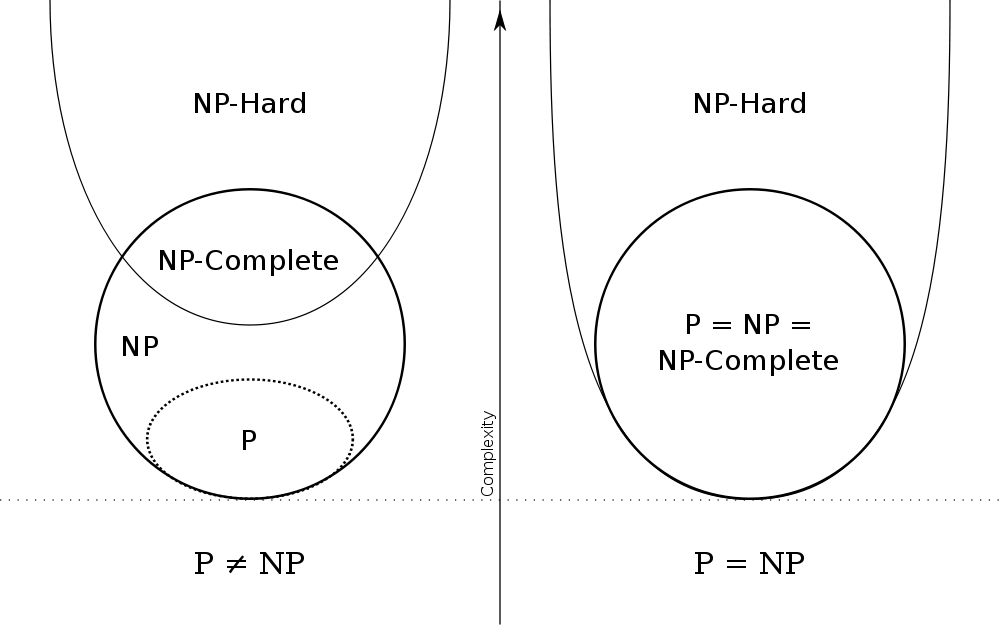
\includegraphics[width=120mm, keepaspectratio]{images/diagramma_classi}		 
		 \end{figure}

\subsection{Ragioni per credere che $P \neq NP$}


Il problema di determinare se $P=NP$	oppure $P \neq NP$ prende il nome di \emph{Problema $P$ vs $NP$}. Ad oggi, nessuno è ancora riuscito a dimostrare una o l'altra tesi. In effetti, \emph{P vs NP} è uno dei più importanti problemi aperti della Matematica e dell'Informatica teorica \footnote{``\emph{It's one of the fundamental mathematical problems of our time, and its importance grows with the rise of powerful computers.}'', Lance Fortnow, The status of the \emph{P} versus \emph{NP} problem, Communications of the ACM 52 (2009), no. 9, pp. 78–86.}, e fa parte dei sette \emph{Problemi per il millennio} del Clay Mathemathics Institute, per la soluzione di ognuno dei quali è stato fissato un premio di un milione di dollari.\\
Al momento, la comunità scientifica sembra propendere per la tesi $P \neq NP$. Nel 2012 William Gasarch, professore di Computer Science alla University of Maryland, ha condotto un sondaggio tra 150 ricercatori a proposito del problema \emph{P} vs \emph{NP}. L'81\% di essi non crede che $P=NP$. Un sondaggio analogo era stato proposto a 100 ricercatori dallo stesso Gasarch nel 2002, e i risultati erano piuttosto diversi: il 61\% non credeva che $P=NP$, il 9\% credeva che P=NP, e il 30\% diceva di non sapere oppure era convinto che il problema non fosse risolvibile \cite{Rosenberger:tesi}.\\
Un altro punto interessante del sondaggio è quello che riguarda i tempi di attesa stimati prima di giungere a una soluzione. Nel 2002, il 62\% degli intervistati sosteneva che una risposta al problema sarebbe arrivata prima del 2100. Nell'ultimo sondaggio, questa percentuale è scesa al 53\%. Gasarch crede che siano necessari persino 200-400 anni. Di seguito riportiamo una sua citazione che spiega brevemente le ragioni di questa convinzione:

``La mia posizione, e francamente la posizione di chiunque, è in realtà un'ipotesi azzardata. Detto questo, la mia impressione è che ci troviamo davvero a un punto morto. Non c'è stato nessun progresso e non c'è nessun vero piano d'attacco.''\cite{Rosenberger:tesi}

C'è da dire che le ragioni per credere che $P \neq NP$ sono diverse. Una di queste è il fatto che dopo decenni di studi sulle classi di complessità e i relativi problemi, nessuno sia stato in grado di trovare un algoritmo che lavori in tempo polinomiale per neanche uno degli oltre 3000 importanti problemi NP-completi conosciuti.\\
Si sostiene anche, dal punto di vista intuitivo, che l'esistenza di problemi che sono difficili da risolvere ma per i quali le soluzioni sono facili da verificare, è in accordo con la nostra esperienza nel mondo reale.\\
D'altra parte, alcuni ricercatori credono che ci sia un'eccessiva sicurezza nel sostenere che $P \neq NP$, e che si dovrebbero considerare anche dimostrazioni di $P=NP$. Ad esempio, nel 2002 Moshe Y. Vardi, delle Rice University, fece questa dichiarazione:

``Il principale argomento a favore della tesi $P \neq NP$ è la totale mancanza di progressi importanti nell'area della ricerca esaustiva. Questo è, a mio parere, un argomento molto debole. La classe degli algoritmi è molto grande e noi siamo solo all'inizio della sua esplorazione. [...] La risoluzione dell'Ultimo Teorema di Fermat mostra che risposte a domande molto semplici possono richiedere teorie estremamente complesse.''\cite{Gasarch:tesi}


\subsection{Conseguenze della risoluzione del problema}

Una delle ragioni per le quali \emph{P} vs \emph{NP} è oggetto di molti studi sta nelle conseguenze di un'eventuale risposta. Qualunque essa sia, costituirebbe un grosso passo avanti per la teoria astratta, e potrebbe anche avere gigantesche conseguenze sul piano applicativo. Ne descriviamo alcune:

\paragraph{Se $P=NP$}\

Una prova che $P=NP$ potrebbe indurre conseguenze pratiche sbalorditive, nel caso in cui la dimostrazione dovesse portare alla scoperta di metodi efficienti per risolvere alcuni dei problemi importanti in \emph{NP}. C'è da dire che questo non è scontato, in quanto la dimostrazione potrebbe essere non-costruttiva (ad esempio, se si mostrasse che supporre $P \neq NP$ porta ad una contraddizione), oppure potrebbe descrivere algoritmi polinomiali, ma di grado troppo alto per essere efficienti nella pratica (cfr. Sezione \ref{commenti_tesi_e-c-k}). In ogni caso, le conseguenze pratiche sarebbero importanti, poiché diversi problemi NP-completi sono fondamentali in numerosi ambiti.\\
\\
La Crittografia, ad esempio, si appoggia fortemente sulla natura ``difficile'' di certi problemi. Una soluzione costruttiva ed efficiente per un problema \emph{NP}-completo come \emph{3SAT} costituirebbe una falla enorme per la maggior parte degli attuali sistemi di crittografia \cite{wikiP=NP:tesi}, inclusi:
\begin{itemize}
\item[-] la crittografia a chiave pubblica, che sta alla base di molte moderne applicazioni in ambito di sicurezza, come le transazioni economiche via Internet; e
\item[-] gli algoritmi a chiave privata, come AES o 3DES, usati per la cifratura dei dati nelle telecomunicazioni.
\end{itemize}

Tutti questi sistemi dovrebbero essere modificati o rimpiazzati con altri che sfruttino principi teorici molto diversi. 

Allo stesso tempo però, ci sarebbero enormi conseguenze positive che seguirebbero dalla capicità di rendere trattabili molti problemi matematici attualmente intrattabili. Ad esempio, numerosi problemi di ricerca operativa sono \emph{NP}-completi, come alcuni tipi di \emph{programmazione intera} e il \emph{problema del commesso viaggiatore}, per fare i nomi di due tra gli esempi più famosi. Soluzioni efficienti per questi problemi avrebbero grandissime implicazioni per la logistica. Altri importanti problemi, come alcuni riguardanti la predizione di struttura proteica, sono anch'essi \emph{NP}-completi; se questi problemi fossero risolvibili in modo efficiente, si potrebbero avere considerevoli vantaggi in Biologia.\\
\\
Ma questi progressi impallidirebbero di fronte alla rivoluzione che un metodo efficiente per risolvere problemi \emph{NP}-completi causerebbe all'interno della Matematica stessa. Secondo Stephen Cook, questo

``trasformerebbe la Matematica, permettendo a un computer di trovare una dimostrazione formale di ogni teorema che ha una dimostrazione di lunghezza ``ragionevole'', dato che le dimostrazioni formali possono essere facilmente verificate in tempo polinomiale [ovvero, le dimostrazioni formali stanno in \emph{NP}]. Sarebbe anche possibile che i teoremi in questione includano tutti i Problemi per il Millennio.''\cite{Cook:tesi}

I matematici che lavorano nella ricerca spendono buona parte del loro tempo cercando di provare teoremi, e alcune dimostrazioni hanno richiesto decenni o anche secoli per essere trovate. Ad esempio, per l'Ultimo Teorema di Fermat sono stati necessari oltre tre secoli. Si capisce quindi come un metodo che garantisca di fornire dimostrazioni per i teoremi (nel caso ne esista una di lunghezza ``ragionevole''), porrebbe essenzialmente fine a queste fatiche.


\paragraph{Se $P \neq NP$}\

Una dimostrazione che $P \neq NP$ non porterebbe gli stessi benefici pratici e computazionali di una prova che $P=NP$, ma implicherebbe allo stesso modo un significativo progresso per la Teoria della computabilità e della complessità, e costituirebbe una guida per ricerche future. Permetterebbe di mostrare in modo formale che molti problemi comuni non possono essere risolti in modo efficiente, autorizzando quindi i ricercatori a focalizzare l'attenzione su soluzioni parziali o soluzioni di altri problemi. Va detto che, in realtà, considerata la diffusa credenza in $P \neq NP$, spesso questa strategia viene già applicata.



\chapter{Macchine di Turing con Oracolo}

\begin{aquote}{Baker, Gill, Solovay \cite{B-G-S:tesi}}
\emph{La domanda P=?NP relativizzata \emph{[agli oracoli]} ha risposta affermativa per alcuni oracoli e negativa per altri. Crediamo che questa sia un'ulteriore prova della difficoltà del problema P vs NP.}
\end{aquote}


\section{Il Teorema di Baker, Gill, Solovay}

Lo scopo di questa sezione è dimostrare un importante risultato dovuto a Baker, Gill, Solovay e spiegare le conseguenze che esso ha sulla Teoria della Complessità e in particolare sul problema \emph{P vs NP}.

\begin{defn}
Sia $T$ una funzione parziale da $\mathbb{N}$ in $\mathbb{N}$. \emph{DTIME}$(T(n))$ è la classe dei linguaggi $S$ su qualche alfabeto finito $A$ per i quali c'è una macchina di Turing deterministica su $A$ che decide $S$ e ha complessità $O(T(n))$.
\end{defn}

\begin{oss}
$P=\cup_{k \in \mathbb{N}}$\emph{DTIME}$(n^k)$
\end{oss}

\begin{defn}
La \emph{classe esponenziale} è $\ex:=\cup_{k \in \mathbb{N}}$\emph{DTIME}$(2^{n^k})$
\end{defn}

Senza perdita di generalità, d'ora in avanti lavoreremo solamente con l'alfabeto binario $A=\{0,1\}$. Ogni oggetto processato da qualsiasi MdT sarà quindi da intendersi come la stringa binaria che lo codifica, anche quando non specificato.\\
\\
Introduciamo adesso le Macchine di Turing con Oracolo. Intuitivamente, le MdT con oracolo sono MdT che hanno accesso a un cosiddetto \emph{oracolo}, che viene trattato come una \emph{black box}, ovvero un oggetto di cui non interessa il funzionamento interno, ma solo il risultato che restituisce, dato un certo input. Più precisamente, un oracolo $O$ è un linguaggio su $\{0,1\}$, e una MdT $M$ con oracolo $O$ è in grado di risolvere ``magicamente'' i prolemi di decisione per $O$ in un singolo passo di computazione. $M$ possiede uno speciale \emph{nastro dell'oracolo} sul quale può scrivere una stringa $w \in \a01$ e ottenere in un solo passo la risposta alla domanda ``$w$ appartiene ad $O$''? La macchina $M$ può accedere all'oracolo un numero arbitrario di volte. Ecco la definizione formale:

\begin{defn}\label{mdt_oracolo}
Una \emph{Macchina di Turing con Oracolo} è una coppia $(M,O)$ dove $O \subseteq \a01$ e $M$ è una Macchina di Turing deterministica con uno speciale \emph{nastro dell'oracolo} e tre speciali stati: $q_?, q_Y, q_N$. Durante la computazione, ogni volta che $M$ entra nello stato $q_?$ e scrive $q \in \a01$ sul \emph{nastro dell'oracolo}, la macchina entra nello stato $q_Y$ se $q \in O$ e $q_N$ se $q \not\in O$. Il procedimento di interrogazione dell'oracolo richiede un solo passo di computazione (va considerato però il tempo richiesto per scrivere $q$ sul \emph{nastro dell'oracolo}).\\
Si usa indicare $(M,O)$ con $M^O$.\\
\\
Le MdT non deterministiche con oracolo si definiscono in modo analogo considerando MdT non deterministiche. Precisiamo però che il ricorso all'oracolo, ovvero la scrittura della stringa $q \in \a01$ sul \emph{nastro dell'oracolo}, viene eseguito in modo deterministico. Ovvero, quando una MdT non deterministica con oracolo entra nello stato $q_?$ deve scrivere sul \emph{nastro dell'oracolo} una stringa $q$ univocamente determinata dai passi di computazione eseguiti fino a quel momento.
\end{defn}


Ricordiamo che quando parliamo di una MdT che \emph{accetta} un linguaggio in tempo limitato rispetto alla lunghezza dell'input da una qualche funzione di complessità, possiamo supporre senza perdita di generalità che la MdT \emph{decida} quel linguaggio, ovvero che converga su ogni input (cfr. Osservazione \ref{decidere=accettare}).

\begin{defn}
Per ogni $O \subseteq \a01$, $P^O$ è l'insieme formato da tutti i linguaggi $L$ per i quali esiste una MdT deterministica con oracolo $O$ che decide $L$ in tempo polinomiale. \emph{NP}$^O$ è l'insieme corrispondente ottenuto considerando MdT non deterministiche con oracolo $O$ (o, equivalentemente, adattando la Definizione \ref{def_NP}, prendendo $S' \in P^O$).
\end{defn}

\begin{oss}\label{card_MdT_oracolo}
È evidente che l'insieme di tutte le MdT con oracolo, intese come coppie $(M,O)$, non è numerabile. Infatti $O$ è un qualsiasi sottoinsieme di $\mathbb{N}$, e sappiamo che $|\mathcal{P}(\mathbb{N})|=|\mathbb{R}|>|\mathbb{N}|$. Consideriamo però l'insieme $\mathcal{M}_o:=\{M : \; (M,O) \text{ è una MdT con oracolo}\}$. È facile convincersi che questo insieme è numerabile, in quanto non è altro che il sottoinsieme di $\mathcal{M}$ formato dalle MdT tradizionali il cui insieme degli stati contiene almeno $q_?$, $q_Y$ e $q_N$. Si conclude ricordando che $\mathcal{M}$ è numerabile (cfr. Teorema \ref{card_mdt}).
\end{oss}

\noindent \textbf{Notazione.} Sia $M$ qualunque una Macchina di Turing deterministica (con o senza oracolo) che decide un linguaggio. Indichiamo con $L(M)$ il linguaggio deciso da $M$. Inoltre, diremo che \emph{M accetta w} se $w \in L(M)$, che \emph{M rifiuta w} altrimenti. Infine, per $x \in \{0,1\}$ e $n \geq 1$, denoteremo con $x^n$ la stringa formata da $x$ ripetuto $n$ volte.

\begin{es}
Con riferimento alla sezione Sezione \ref{SAT}, sia $\overline{SAT}$ il linguaggio formato dagli insiemi di clausole che non sono soddisfacibili. Allora $\overline{SAT} \in P^{SAT}$. Infatti, per ogni insieme di clausole $w$ è possibile controllare se $w \in \overline{SAT}$ in due soli passi di computazione (più quelli necessari per scrivere $w$ sul \emph{nastro dell'oracolo}), grazie all'oracolo: al primo passo si chiede all'oracolo se $w \in SAT$, al secondo passo si inverte la risposta.
\end{es}

Descriviamo adesso un linguaggio che ha un ruolo cruciale nella dimostrazione del Teorema di Baker, Gill, Solovay.

\begin{defn}
Chiamiamo $\ec$ il linguaggio\\
\\
\centerline{$\{(M,x,k) : \; x \in \a01, \, k \in \mathbb{N} \,$ e $M$ è una MdT deterministica}\\ 
\centerline{tale che $M \downarrow x$ con output ``\emph{SÌ}'' entro $k$ passi$\}$}
\end{defn}

\begin{lemma}\label{lemma_oracoli}
$P^{\ec}=NP^{\ec}$
\begin{proof}
Proviamo che
$$\ex \subseteq P^{\ec} \subseteq NP^{\ec} \subseteq \ex$$
\begin{enumerate}
\item Mostriamo la prima inclusione: sia $S \in \ex$. Siano $h \in \mathbb{N}$ e $M$ una MdT che decide $S$ e ha complessità $c \cdot 2^{n^h}$ per qualche $c>0$. Simuliamo allora ogni computazione di $M$ su qualsiasi input $w$ con $M_S^{\ec}$, la MdT deterministica con oracolo $\ec$ che si comporta nel seguente modo: quando $M_S^{\ec}$ deve processare $w$, chiede all'oracolo se $(M,w,k) \in \ec$, dove $k:=c \cdot 2^{|w|^h}$.\footnote{È importante osservare che quanto appena detto è lecito, ovvero che $M_S^{\ec}$ può effettivamente scrivere $k=c \cdot 2^{|w|^h}$ sul \emph{nastro dell'oracolo} in tempo polinomiale rispetto a $|w|$. Questo è vero perché la lunghezza di $k$, scritto in codifica binaria, è $1+\lfloor \log_2 k \rfloor=1+\lfloor \log_2 \left(c \cdot 2^{|w|^h}\right) \rfloor= O(|w|^h)$.} È evidente che $M_S^{\ec}$ decide $S$ (in quanto per ogni $w$ l'oracolo risponde lo stesso output di $M$ su $w$), e per ogni $w$ la computazione richiede un solo passo (più quelli necessari per la scrittura di $(M,w,k)$ sul \emph{nastro dell'oracolo}), indipendentemente dall'input. Quindi $S=L(M_S^{\ec})$ e $L(M_S^{\ec}) \in P^{\ec}$. Perciò $S \in P^{\ec}$.

\item La seconda inclusione è immediata (il Teorema \ref{P_in_NP} si estende banalmente alle MdT con oracolo).

\item Mostriamo che $NP^{\ec} \subseteq \ex$. Sia quindi $S \in NP^{\ec}$. Allora, secondo la Definizione \ref{mdt_oracolo} (che si rifà alla Definizione \ref{def_NP}), esistono una MdT deterministica $M_S^{\ec}$ con oracolo $\ec$ e due polinomi $p_S, t_S$ tali che, per ogni $w \in \a01$,
\begin{itemize}
\item $w \in S$ se e solo se esiste $y \in \a01$ per cui $|y| \leq p_S(|w|)$ e $M_S^{\ec}$ converge su $w \star y$;
\item su ogni possibile input, $M_S^{\ec}$ converge in tempo al più polinomiale limitato da $t_s$ rispetto alla lunghezza dell'input stesso, e termina con output \emph{``SÌ''} oppure \emph{``NO''}.
\end{itemize}
Costruiamo allora una MdT deterministica $M$ come segue: per ogni $w \in \a01$, 
\begin{itemize}
\item $M$ genera prima tutte le stringhe $y$ con $|y| \leq p_S(|w|)$,
\item $M$ simula poi $M_S^{\ec}$ su ogni stringa $w \star y$.
\end{itemize}
Chiaramente $M$ decide $S$, ovvero $L(M)=S$. Affermiamo che $M$ ha complessità $O(2^{n^h})$ per qualche $h \in \mathbb{N}$. Infatti:
\begin{itemize}
\item[a)] $M$ scrive tutte le stringhe binarie $y$ di lunghezza $\leq p_S(|w|)$, che sono in numero $2^{p_S(|w|)+1}-1$;
\item[b)] $M$ esegue poi, per ogni $y$, la computazione di $M_S^{\ec}$ su $w \star y$, che ha un numero di passi polinomiale, limitato da $t_S$;
\item[c)] Resta da discutere quanto impiega $M$ a svolgere i compiti che $M_S^{\ec}$ assegna all'oracolo. Per ogni $y$ con $|y| \leq p_S(|w|)$, $M_S^{\ec}$ può ricorrere all'oracolo un numero al più polinomiale di volte, limitato anch'esso da $t_S$ (altrimenti impiegherebbe troppi passi per scrivere tutti gli input sul \emph{nastro dell'oracolo}). A questo punto, basta osservare che una singola chiamata all'oracolo $\ec$ con input $(M',x,k)$ può essere simulata da $M$ in un numero di passi costante (ovvero al più $k$ passi).\footnote{NB: tutti gli $(M',x,k)$ che $M_S^{\ec}$ propone all'oracolo devono necessariamente avere lunghezza polinomiale rispetto a $|w|$, perché altrimenti il tempo necessario per scriverli sul \emph{nastro dell'oracolo} supererebbe il limite imposto da $t_S$.}
\end{itemize}
In conclusione, $M$ ha come complessità una funzione che è prodotto e composizione di polinomi e di esponenziali, tale comunque da rientrare nella classe $O(2^{n^h})$ per qualche $h \in \mathbb{N}$. Quindi $L(M) \in \ex$, ovvero $S \in \ex$.
\end{enumerate}
\end{proof}
\end{lemma}

Possiamo ora enunciare e dimostrare il teorema di Baker, Gill e Solovay del 1975 \cite{B-G-S:tesi}. Spiegheremo poi l'importanza di questo risultato.

\begin{teo}[Baker, Gill, Solovay]\
\begin{enumerate}
\item Esiste un oracolo $A$ tale che $P^A=NP^A$.
\item Esiste un oracolo $B$ tale che $P^B \neq NP^B$.
\end{enumerate}

\begin{proof}
Per il primo punto, è sufficiente prendere $A:=\ec$ e ricordare il Lemma \ref{lemma_oracoli}.\\
La dimostrazione del secondo punto sfrutta un classico argomento di diagonalizzazione. Costruiremo un oracolo $B \subseteq \a01$ per il quale $P^B \neq NP^B$. Per ogni $n \in \mathbb{N}$, l'oracolo $B$ conterrà al più una stringa di lunghezza $n$, che spiegheremo come determinare. Considereremo poi il linguaggio 
$$L:=\{0^i | \; B \text{ contiene una parola di lunghezza } i\}$$
Possiamo facilmente costruire una MdT non deterministica con oracolo $B$ tale che, dato $0^i$ come input, genera non deterministicamente una stringa in $\a01$ di lunghezza $i$, la sottopone all'oracolo $B$, e la accetta se e solo se l'oracolo risponde ``SÌ''. Quindi $L \in NP^B$. D'altra parte, costruiremo $B$ in modo tale che ogni sua stringa di qualunque lunghezza (se presente), sarà talmente ``nascosta'' che nessuna MdT deterministica con oracolo $B$ sarà in grado di trovarla in tempo polinomiale. Procediamo allora con la dimostrazione, nella quale i logaritmi coinvolti sono tutti da intendersi con base 2.\\
Vogliamo costruire l'insieme $B$ come unione di insiemi $B_i$ con $i \geq 1$ tali che $B_i \subseteq B_{i+1}$ per ogni $i \geq 1$. Come già detto, l'insieme $B$ conterrà al più una stringa di ogni lunghezza. Mentre generiamo gli insiemi $B_i$, costruiamo anche degli insiemi $V_i$ di stringhe ``vietate'', nel senso che necessariamente non potranno appartenere a $B$. Anche gli insiemi $V_i$ saranno tali da soddisfare $V_i \subseteq V_{i+1}$ per ogni $i \geq 1$.\\


Fissiamo un'enumerazione $(M_{i+1})_{i \in \mathbb{N}}$ di tutte le MdT deterministiche con oracolo sull'alfabeto binario (si veda l'Osservazione \ref{card_MdT_oracolo}). Supponiamo inoltre che, nella fissata enumerazione, ogni MdT compaia un numero infinito di volte \footnote{Chi dovesse nutrire qualche dubbio riguardo all'esistenza di una enumerazione con questa caratteristica, ricordi che $\mathbb{N} \times \mathbb{N} \approx \mathbb{N}$.}.\\
Ci proponiamo di definire un oracolo $B$ ``a stadi''. Simultaneamente alla costruzione di $B$, sempre a stadi, procediamo alla costruzione di un insieme $V$ di stringhe ``vietate'', che necessariamente non dovranno appartenere a $B$.\\
Formalmente, vogliamo definire in modo ricorsivo due successioni $(B_{i+1})_{i \in \mathbb{N}}$ e $(V_{i+1})_{i \in \mathbb{N}}$ con le proprietà che:
\begin{enumerate}
\item[(1)] $B_1=V_1=\emptyset$;
\item[(2)] $B_i \subseteq B_{i+1}$ per ogni $i \geq 1$;
\item[(3)] $V_i \subseteq V_{i+1}$ per ogni $i \geq 1$;
\item[(4)] $B_i \cap V_i = \emptyset$ per ogni $i \geq 1$;
\item[(5)] Per ogni $i \geq 1$ e per ogni $0 \leq k < i$, $B_i$ contiene al più una stringa di lunghezza $k$;
\item[(6)] Per ogni $i \geq 1$, allo stadio $i$ potrà essere aggiunta a $B_i$ al più una stringa $b_i$, che dovrà necessariamente essere di lunghezza $i$. In tal caso, si porrà $B_{i+1}:=B_i \cup \{b_i\}$.
\end{enumerate}
Gli insiemi $B$ e $V$ verranno infine così definiti: $B:=\cup_{i \in \mathbb{N}} B_{i+1}$ e $V:=\cup_{i \in \mathbb{N}} V_{i+1}$.\\
\noindent Ecco finalmente i dettagli della procedura.\\
\\
Sia $i \geq 1$. Suppponiamo di aver definito $(B_j)_{0<j \leq i}$ e $(V_j)_{0<j \leq i}$ che soddisfano le condizioni $(1)\dot{-}(6)$ per ogni $0<j \leq i$. Al passo $i$-esimo ci proponiamo di definire $B_{i+1}$ e $V_{i+1}$ in modo che $(1)\dot{-}(6)$ valgano per ogni $0<j \leq i+1$. Vediamo come.\\
Allo stadio $i$-esimo, con $i \geq 1$, simuliamo $M_i^{B_i}$ sull'input $0^i$. Se, durante la computazione di $M_i^{B_i}$ sull'input $0^i$, $M_i^{B_i}$ si trova nella situazione di dover proporre all'oracolo una stringa $w$ di lunghezza $<i$, allora semplicemente consultiamo l'oracolo $B_i$ relativamente a $w$. Se $M_i^{B_i}$ deve proporre all'oracolo qualche stringa $y$ con $|y| \geq i$, aggiungiamo $y$ a $V_i$, etichettandola quindi come ``stringa vietata''.\\
La simulazione di $M_i^{B_i}$ su $0^i$ continua per $i^{\log i}$ passi, al termine dei quali sono state eventualmente etichettate alcune stringhe come ``vietate''. Definiamo $V_{i+1}$ come l'insieme ottenuto aggiungendo queste stringhe a $V_i$. Inoltre, dopo $i^{\log i}$ passi, indipendentemente dal fatto che $M_i^{B_i}$ abbia terminato o meno la sua computazione, prendiamo una decisione riguardo alla formazione dell'insieme $B_{i+1}$. Se entro $i^{\log i}$ passi, $M_i^{B_i}$ si è fermata e ha rifiutato $0^i$, allora formiamo l'insieme $B_{i+1}$, aggiungendo a $B_i$ una stringa $b_i$ di lunghezza $i$ che non sia nell'insieme $V_{i+1}$ di quelle vietate \footnote{Si osservi che a questo punto della procedura, l'insieme delle stringhe vietate da considerare è $V_{i+1}$, che contiene anche tutte le stringhe di lunghezza $\geq i$ eventualmente proposte all'oracolo da $M_i^{B_i}$.}, ammesso che una tale stringa esista. La stringa in questione può essere scelta in modo arbitrario. Se $M_i^{B_i}$ non rifiuta $0^i$ entro $i^{\log i}$ passi, poniamo $B_{i+1}:=B_i$ (e quindi $B$ non conterrà mai una stringa di lunghezza $i$).\\
Notiamo che è possibile che non esista alcuna stringa di lunghezza $i$ in $B$ se tutte le stringhe di lunghezza $i$ sono state etichettate come ``vietate'' entro la fine della simulazione di $M_i^{B_i}$. Osserviamo però che, per ogni $j$, $M_j^{B_j}$ viene simulata per $j^{\log j}$ passi, quindi la cardinalità di $V_{i+1}$ non supera
$$\sum_{j=1}^i j^{\log j} \leq i \cdot i^{\log i} = i^{i+\log i}.$$
Poiché ci sono $2^i$ stringhe binarie di lunghezza $i$, siamo sicuri che non tutte le stringhe di lunghezza $i$ sono vietate se $2^i > i^{1+\log i}$, ovvero se $i > (1+\log i) \log i$. Quest'ultima disequazione è soddisfatta per ogni $i \geq 32$, quindi c'è solo un piccolo insieme di indici $i$ per i quali tutte le stringhe di lunghezza $i$ possono essere vietate.\\
\\
È evidente che gli insiemi $B_{j}$ e $V_{j}$ così costruiti assicurano la validità di $(1)\dot{-}(6)$ per ogni $0 < j \leq i+1$.\\
\\
Proviamo ora che
$$L:=\{0^i | \; B \text{ contiene una parola di lunghezza } i\}$$
appartiene a $NP^B \setminus P^B$.\\
Come abbiamo osservato all'inizio della dimostrazione, $L \in NP^B$.\\
Mostriamo che $L \not\in P^B$. Procediamo per assurdo. Siano $k \geq 1$ e $p(n)$ un polinomio tali che $M_k^B$ decide $L$ e ha complessità $p(n)$. Poiché, nella nostra enumerazione, ogni MdT compare un numero infinito di volte, possiamo supporre senza perdita di generalità $k \geq 32$ e $k^{\log k} \geq p(k)$. Allora:
\begin{itemize}
\item[-] Se $M_k^B$ accetta $0^k$, allora $0^k \in L$ e quindi, per definizione di $L$, $B$ contiene una stringa di lunghezza $k$. Per come abbiamo costruito $B$, questo significa che $M_k^{B_k}$ rifiuta $0^k$. D'altra parte, $M_k^B$ e $M_k^{B_k}$ svolgono due computazioni assolutamente identiche su $0^k$, in quanto $B$ e $B_k$ contengono esattamente le stesse stringhe di lunghezza $<k$, e $B$ non contiene nessuna stringa di lunghezza $\geq k$ che viene proposta all'oracolo da $M_k^{B_k}$ nella computazione su $0^k$ (perché allo stadio $k$ tutte le stringhe di questo tipo\footnote{ovvero le stringhe di lunghezza $\geq k$ che vengono proposte all'oracolo $B_k$ da $M_k^{B_k}$ durante la computazione di $M_k^{B_k}$ su $0^k$.} erano state etichettate come vietate e inserite in $V_{k+1}$). Quindi $M_k^B$ rifiuta $0^k$, e abbiamo una contraddizione.
\item[-] Se $M_k^B$ rifiuta $0^k$, allora $0^k \not\in L$. Ma ciò significa che $M_k^{B_k}$ non rifiuta $0^k$ entro $k^{\log k}$ passi. Questo deriva dal fatto che $k \geq 32$, e se $M_k^{B_k}$ rifiutasse $0^k$ entro $k^{\log k}$ passi, allora esisterebbe almeno una stringa di lunghezza $k$ che non è stata inserita tra quelle vietate, e quindi $B$ ne conterrebbe una, ovvero $0^k$ apparterrebbe a $L$. Perciò $M_k^{B_k}$ non rifiuta $0^k$ entro $k^{\log k}$ passi, e quindi nemmeno $M_k^B$. Ma poiché $k^{\log k} \geq p(k)$, $M_k^B$ termina la sua computazione su $0^k$ entro $k^{\log k}$ passi e quindi non rifiuta $0^k$ in assoluto, e si arriva di nuovo a una contraddizione.
\end{itemize}
Quindi $M_k^B$ accetta $0^k$ se e solo se $M_k^B$ rifiuta $0^k$.\\
Concludiamo che $L \in NP^B \setminus P^B$, ovvero $P^B \neq NP^B$.
\end{proof}
\end{teo}

\paragraph{Commenti sul Teorema di Baker, Gill, Solovay}\ \\
Il Teorema di Baker, Gill, Solovay ha profonde ripercussioni sulla ricerca di una strategia per risolvere il problema \emph{P vs NP}. Esistono diversi metodi per confrontare due classi di complessità. Il Teorema di B-G-S ci dice che alcuni tra quelli più usati fallirebbero se sfruttati per risolvere il problema \emph{P vs NP}.\\
Siano $A$ e $B$ gli oracoli della dimostrazione del Teorema di B-G-S.\\
Una tecnica per mostrare che due classi di complessità $X, Y$ sono uguali è la \emph{simulazione} di ogni MdT di $X$ con una MdT di $Y$ (e viceversa). Ne abbiamo visto un semplice esempio nella dimostrazione del Lemma \ref{lemma_oracoli}. Supponiamo ora di voler simulare una MdT non deterministica che decide un arbitrario problema \emph{NP}-completo mediante una MdT deterministica con complessità polinomiale (ricordando il Teorema \ref{teo_NP-completo}, l'esistenza di una tale MdT proverebbe che $P=NP$). Sembra plausibile che la simulazione in questione continui a funzionare anche se dotiamo entrambe le MdT di uno stesso oracolo. Ma se come oracolo scegliamo $B$, otteniamo che $P^B = NP^B$, e abbiamo appena provato che ciò è falso.\footnote{Altri esempi di simulazioni che vengono preservate se relativizzate a un qualsiasi oracolo sono tutte quelle usate nel Capitolo 7 di \cite{Ullman:tesi}.}\\
Un metodo per mostrare che due classi sono diverse è quello della diagonalizzazione, usato ad esempio nella dimostrazione del Teorema di B-G-S (per altri esempi si veda \cite[Teorema 12.8 e 12.9]{Ullman:tesi}). Anche la diagonalizzazione tende a restare valida in presenza di oracoli. Se provassimo a usare la diagonalizzazione sulla classe $P$ per mostrare che un certo linguaggio sta in $NP \setminus P$, allora la stessa dimostrazione probabilmente potrebbe anche provare che $NP^A \setminus P^A \neq \emptyset$, contraddicendo il Teorema di B-G-S.\\
Infine, si può tentare di sfruttare delle proprietà di chiusura per trovare differenze tra due classi, mostrando quindi che sono diverse. Un esempio è la chiusura rispetto al complementare. Potremmo cercare una proprietà di chiusura di $P$ che non è valida anche per $NP$? Questo può sembrare uno degli approcci più promettenti. Infatti, una dimostrazione che $P$ è chiuso rispetto a qualche operazione, probabilmente continuerebbe ad essere valida anche per $P^A$. Al contrario, una determinata proprietà di chiusura non soddisfatta da $NP$ potrebbe invece valere per $NP^A$. Quindi questa potrebbe rivelarsi una direzione d'indagine promettente. D'altra parte, mostrare che $NP$ non è chiuso rispetto a una certa operazione richiederebbe verosimilmente di provare che un particolare linguaggio non appartiene a $NP$. Una dimostrazione di questo tipo potrebbe sfruttare la diagonalizzazione, ma come già detto, questa probabilmente continuerebbe a valere anche per $NP^A$. Si potrebbe anche sviluppare un argomento \emph{ad-hoc} che non sfrutti nessuna delle tecniche ``classiche'' appena descritte, ma ciò sembra richiedere capacità e conoscenze che vanno oltre quelle attuali.\\
In conclusione, il Teorema di Baker, Gill, Solovay fornisce un'ulteriore conferma della difficoltà del problema \emph{P vs NP}.


\section{Indipendenza di $P=NP$ da \emph{ZF} relativamente a un Oracolo}

Vogliamo dare un cenno della dimostrazione di un teorema del 1979 dovuto a Hartmanis e Hopcroft \cite{Hopcroft:tesi}. Il risultato in questione afferma che esiste un oracolo $O$ tale che $P^O=NP^O$ non è decidibile nel sistema di assiomi di Zermelo-Fraenkel, ovvero, sotto l'ipotesi di consistenza di \emph{ZF}, $P^O=NP^O$ non è dimostrabile né refutabile (i.e. dimostrabile la negazione) in \emph{ZF}. La dimostrazione sfrutta due importanti risultati di Teoria della Computabilità: il Teorema S-m-n e il Teorema di Ricorsione. Decidiamo di non trattarli in questo elaborato, in quanto al di fuori dei nostri scopi. Chi fosse interessato può trovarli in \cite{Cutland:tesi}. 

\begin{lemma}\label{lemma_oracoli_tagliati}
Siano $A$ e $B$ gli oracoli del teorema di Baker-Gill-Solovay. Siano $\{a_0,...,a_n\} \subset A$ e $\{b_0,...,b_m\} \subset B$. Siano $A':= A \setminus \{a_0,...,a_n\}$ e $B':= B \setminus \{b_0,...,b_m\}$. Allora valgono
\begin{enumerate}
\item $P^{A'}=NP^{A'}$
\item $P^{B'} \neq NP^{B'}$
\end{enumerate}
\begin{proof}\
\begin{enumerate}
\item Procediamo per assurdo. Sia $S \in NP^{A'} \setminus P^{A'}$. Poiché $S \in NP^{A'}$ e $A' \subset A$, si ha $S \in NP^A$. Inoltre $NP^A=P^A$, quindi $S \in P^A$, ovvero esiste una MdT deterministica $M_S^A$ tale che $L(M_S^A)=S$ e $M_S^A$ ha complessità polinomiale $c_{M_S^A}(l)$, dove $l$ è la lunghezza dell'input. Sia $M'$ una MdT deterministica (senza oracolo) che decide $\{a_0,...,a_n\}$ con complessità $c_{M'}$ (una tale $M'$ esiste perché qualsiasi insieme finito è banalmente decidibile). Sia $k:= \sum_{i=0}^n c_{M'}(|a_i|)$. Allora possiamo costruire una MdT deterministica $M^{A'}$ che si comporta in questo modo: $M^{A'}$ svolge la stessa computazione di $M_S^A$, ma quando $M_S^A$ si trova nella situazione di dover interpellare l'oracolo $A$ relativamente a qualche $a_i$ con $0 \leq i \leq n$, allora $M^{A'}$ simula $M'$ su $a_i$ finché la computazione di $M'$ su $a_i$ non termina, e riprende poi la simulazione di $M_S^A$ dove l'aveva lasciata. È evidente che $L(M^{A'})=S$ e che $c_{M^{A'}}(l) \leq c_{M_S^A}(l) + k$ per ogni $l \in \mathbb{N}$. Poiché $c_{M_S^A}(l) + k$ è polinomiale in $l$, abbiamo una contraddizione.
\item Procediamo per assurdo. Supponiamo allora $P^{B'}=NP^{B'}$. Sia $S \in NP^B \setminus P^B$. Poiché $B'= B \setminus \{b_0,...,b_m\}$, è facile costruire una MdT non deterministica con oracolo $M^{B'}$ che decide $S$ in tempo polinomiale (si costruisce in modo simile a $M^{A'}$ del punto 1). Quindi $S \in NP^{B'}$. Ma allora $S \in P^{B'}$, e poiché $B' \subset B$ allora $S \in P^B$, e abbiamo una contraddizione.
\end{enumerate}
\end{proof}
\end{lemma}


\begin{teo}[Hartmanis-Hopcroft]
Esiste una Macchina di Turing $M$ che converge su ogni input, tale che né $P^{L(M)}=NP^{L(M)}$ né $P^{L(M)} \neq NP^{L(M)}$ è dimostrabile in \emph{ZF}, assumendo \emph{ZF} consistente.
\begin{proof}
Per semplicità, in questa dimostrazione supponiamo di avere fissato una codifica biiettiva e effettiva tra l'insieme di tutte le stringhe sull'alfabeto binario e l'insieme dei numeri naturali.\\
Siano $A$ e $B$ gli oracoli del teorema di Baker-Gill-Solovay. Fissiamo un'enumerazione $(P_{j+1})_{j \in \mathbb{N}}$ di tutte le dimostrazioni in \emph{ZF}. Il Teorema S-m-n e il Teorema di Ricorsione assicurano l'esistenza di una Macchina di Turing deterministica (senza oracolo) $M$ che si comporta nel seguente modo. Sia $x$ un numero naturale $\geq 1$. $M$ accetta $x$ se e solo se vale una (e una sola) delle seguenti:
\begin{enumerate}
\item[(1)] $x \in B$ ed esiste $1 \leq k \leq x$ tale che $P_k$ è una dimostrazione di $P^{L(M)}=NP^{L(M)}$;
\item[(2)] $x \in A$ ed esiste $1 \leq k \leq x$ tale che $P_k$ è una dimostrazione di $P^{L(M)} \neq NP^{L(M)}$.
\end{enumerate}
Supponiamo adesso che in \emph{ZF} esista una dimostrazione che $P^{L(M)}=NP^{L(M)}$. Sia $m:=\min \{x \in B: \text{ esiste } 1 \leq i \leq x \text{ tale che } P_i \text{ è una dimostrazione di } P^{L(M)}=NP^{L(M)}\}$. È evidente che $L(M)=B \setminus \{0,...,m-1\}$, ovvero $L(M)$ coincide con $B$ tranne che per un numero finito di elementi. Quindi, per il Lemma \ref{lemma_oracoli_tagliati}, $P^{L(M)} \neq NP^{L(M)}$.\\
Viceversa, supponiamo che in \emph{ZF} esista una dimostrazione che $P^{L(M)} \neq NP^{L(M)}$. Sia $m:=\min \{x \in A:  \text{ esiste } 1 \leq i \leq x \text{ tale che } P_i \text{ è una dimostrazione di } P^{L(M)} \neq NP^{L(M)}\}$. È evidente che $L(M)=A \setminus \{0,...,m-1\}$, ovvero $L(M)$ coincide con $A$ tranne che per un numero finito di elementi. Quindi, per il Lemma \ref{lemma_oracoli_tagliati}, $P^{L(M)}=NP^{L(M)}$.\\
Concludiamo che, assumendo \emph{ZF} consistente, non esiste una dimostrazione che $P^{L(M)}=NP^{L(M)}$ o $P^{L(M)} \neq NP^{L(M)}$.
\end{proof}
\end{teo}








%%%%%%%%%%%%%%%%%%%%%%%%%%%%%%%%%%%%%%%%%%%%%%%%%%%%%%%%%%%%
%bibliografia
\cleardoublepage
\addcontentsline{toc}{chapter}{\bibname}

\begin{thebibliography}{3}

\bibitem{Toffalori:tesi}
Carlo Toffalori, Flavio Corradini, Stefano Leonesi, Stefano Mancini (2005),
\emph{Teoria della computabilità e della complessità}, McGraw-Hill, Milano

\bibitem{wikiP=NP:tesi}
P versus NP problem. (2013, September 1). In \emph{Wikipedia, The Free Encyclopedia}. Retrieved 14:50, September 1, 2013, from \url{http://en.wikipedia.org/w/index.php?title=P_versus_NP_problem&oldid=570667214}

\bibitem{Rosenberger:tesi}
Rosenberger, Jack (May 2012). ``P vs. NP poll results''. \emph{Communications of the ACM} 55 (5): 10. \url{http://mags.acm.org/communications/201205?pg=12#pg12}

\bibitem{Gasarch:tesi}
William I. Gasarch (June 2002). ``The P=?NP poll''. SIGACT News 33 (2): 34–47.
\url{http://dl.acm.org/citation.cfm?doid=1052796.1052804}

\bibitem{Cook:tesi}
Cook, Stephen (April 2000). ``The P versus NP Problem''. Clay Mathematics Institute. 
\url{http://www.claymath.org/millennium/P_vs_NP/pvsnp.pdf}

\bibitem{Arora:tesi}
Sanjeev Arora, Boaz Barak (2009), \emph{Computational Complexity: a modern approach}, Cambridge University Press, New York

\bibitem{Ullman:tesi}
John E. Hopcroft, Jeffrey D. Ullman (1979), \emph{Introduction to automata theory, languages and computation}, Addison-Wesley Publishing Company

\bibitem{B-G-S:tesi}
T. Baker, J. Gill, R.Solovay (1975), \emph{Relativizations of the P=?NP question}, SIAM J. Comput

\bibitem{Aaronson:tesi}
Scott Aaronson, \emph{Is P Versus NP Formally Independent?}. 
\url{www.scottaaronson.com/papers/pnp.pdf}

\bibitem{Hopcroft:tesi}
J. Hartmanis and J. Hopcroft, \emph{Independence results in computer science}, SIGACT News 8(4):13–24, 1976.
\url{http://dl.acm.org/citation.cfm?id=1008336}

\bibitem{Cutland:tesi}
N. J. Cutland (1980), \emph{Computability : an introduction to recursive function theory}, Cambridge University Press, New York

\end{thebibliography}




\end{document}
